


\documentclass{article}

\usepackage{amsmath, bm}
\usepackage{graphicx}
\usepackage{amssymb}
\usepackage{float}
\usepackage{caption}
\usepackage{subcaption}
\usepackage{hyperref}
\usepackage{tikz}
\usepackage{pgfplots}
\usepackage{enumitem}
\usepackage{hyperref}
\usepackage{tikz}
\usepackage{pgfplots}
\usepackage{listings}
\usepackage{xcolor}
\usepackage[margin=1in]{geometry}
\usepackage{savetrees}

% Custom subsection numbering
\renewcommand{\thesubsection}{\roman{subsection})}
\renewcommand{\thesubsubsection}{\alph{subsubsection})}

% Set depth for numbering and TOC
\setcounter{secnumdepth}{3}
\setcounter{tocdepth}{3}

% Explicit formatting with indentation
\usepackage{titlesec}

% Indent subsection titles (Roman numerals)
\titleformat{\subsection}
  {\normalfont\normalsize\bfseries}
  {\hspace{1.5em}\thesubsection}{1em}{}

% Indent subsubsection further (nested under subsection)
\titleformat{\subsubsection}
  {\normalfont\normalsize\itshape}
  {\hspace{2em}\thesubsubsection}{1em}{}

\usetikzlibrary{calc}
\usetikzlibrary{angles,quotes} % for pic
\usetikzlibrary{patterns,snakes}
\usetikzlibrary{arrows}
\usetikzlibrary{shapes.geometric, arrows}
\tikzset{>=latex} % for LaTeX arrow head

\setlength{\parskip}{\baselineskip}%
\setlength{\parindent}{0pt}%
\linespread{0.9}


\lstset{
  language=Matlab,
  basicstyle=\ttfamily\small,
  keywordstyle=\color{blue}\bfseries,
  commentstyle=\color{green!60!black},
  stringstyle=\color{orange},
  numbers=left,
  numberstyle=\tiny\color{gray},
  stepnumber=1,
  numbersep=10pt,
  breaklines=true,
  backgroundcolor=\color{gray!10},
  captionpos=b
}
\tikzset{
    cg/.style={
        draw,
        circle,
        thick,
        minimum size=0.2cm, % Adjust the size of the circle
        inner sep=0,      % Remove extra padding
        append after command={
            \pgfextra{
                \draw[thick] (\tikzlastnode.south) -- (\tikzlastnode.north);
                \draw[thick] (\tikzlastnode.west) -- (\tikzlastnode.east);
            }
        }
    }
}

\tikzstyle{startstop} = [rectangle, rounded corners, minimum width=3cm, minimum height=1cm,text centered, draw=black, fill=red!30]
\tikzstyle{process} = [rectangle, minimum width=3cm, minimum height=1cm, text centered, draw=black, fill=orange!30]
\tikzstyle{decision} = [diamond, minimum width=3cm, minimum height=1cm, text centered, draw=black, fill=green!30]
\tikzstyle{io} = [trapezium, trapezium left angle=70, trapezium right angle=110, minimum width=3cm, minimum height=1cm, text centered, draw=black, fill=blue!30]
\tikzstyle{arrow} = [thick,->,>=stealth]

\begin{document}

\title{4F2 Robust and Nonlinear control}
%\title{PRE EAMC DEADLINE DO NOT MARK}
\author{5735G}
\date{March 2025}
\maketitle 

\begin{center}
    \textbf{Summary} \\
    This report covers the analysis and design of nonlinear control systems using linear matrix inequalities (LMIs) and scaled relative graphs (SRGs).
    It begins with stabilizing and oscillatory behavior in recurrent neural networks, presenting conditions for bounded differential gain, autonomous nonlinear oscillations, enforced 2-dominance, and instability of the zero equilibrium.
    These methods are applied to a small robotic insect model, examining excess output passivity and the design of oscillator weights for input passivity shortage.
    Closed-loop dominance is analyzed using passivity theorems. 
    A periodic input-driven contractive network is then introduced to replicate the oscillator's behavior.
    The second half of the report addresses pharmacokinetics and drug dosage control using scaled relative graphs (SRGs), covering both single-compartment and positive feedback models.
    Finally, automatic drug dosing strategies are considered with and without sensor dynamics, including a delay model analyzed via describing function methods.
\end{center}

\section{Stable and oscillatory recurrent neural networks}

\begin{equation}
    \dot{x} = Ax + f(u) + B_w w = \begin{bmatrix}
        -10 & 0 & 10 \\
        0 & -100 & 100 \\
        0 & 0 & -1
    \end{bmatrix} x + \begin{bmatrix}
        0 \\ 0 \\ \varphi(u)
    \end{bmatrix} + \begin{bmatrix}
        0 \\ 0 \\ 1
    \end{bmatrix} r
\end{equation}

\begin{equation}
    y = Cx + D_u u + D_w w = y
\end{equation}

And the feedback interconnection $u = w x$ is used to form the closed loop system.

The nonlinear activation function is defined as $\varphi(x) = \tanh(x)$ Jacobians are defined as

\subsection{Weights to satisfy a bounded differential gain}

The derivative $\varphi'$ acts like a sigmoid which satisfies the condition
\begin{equation}
    0 \leq \varphi'(x) \leq 1 \quad \forall x \in \mathbb{R}
\end{equation}

This allows us to define a complex hull which contains $\partial f(x)$:

\begin{equation}
    \partial f(x) \in \{ B_0 + sB_1 | s \in [0,1]\}
\end{equation}

This allows us to define two linear matrix inequalities (LMIs) to guarantee differential gain. 

\textit{p}-gain $\gamma$ from $w$ to $y$ with rate $\lambda \geq 0$: find $Y = Y^T$ with inertia $p$, $Z$, and $\varepsilon > 0$,

\begin{equation}
    \left[
    \begin{array}{ccc}
    Y \partial f(x)^T + \partial f(x) Y + 2 \lambda Y + Z^T B_u^T + B_u Z + \varepsilon I & B_w & YC^T \\
    B_w^T & -\gamma I & D_w^T \\
    CY & D_w & -\gamma I
    \end{array}
    \right] \leq 0
\end{equation}
\begin{equation}
    \left[
    \begin{array}{ccc}
    Y \partial f(x)^T + \partial f(x) Y + 2 \lambda Y + \varepsilon I & B_w & YC^T \\
    B_w^T & -\gamma I & D_w^T \\
    CY & D_w & -\gamma I
    \end{array}
    \right] \leq 0
\end{equation}

Where the weights are calculated by $W = ZY^{-1}$.
For a $\lambda = 0.1$ the LMI is solved using CVX and the weights are calculated as $W =$ \texttt{[2.8670   42.2303  -48.7531]}.

\begin{figure}[H]
    \centering
    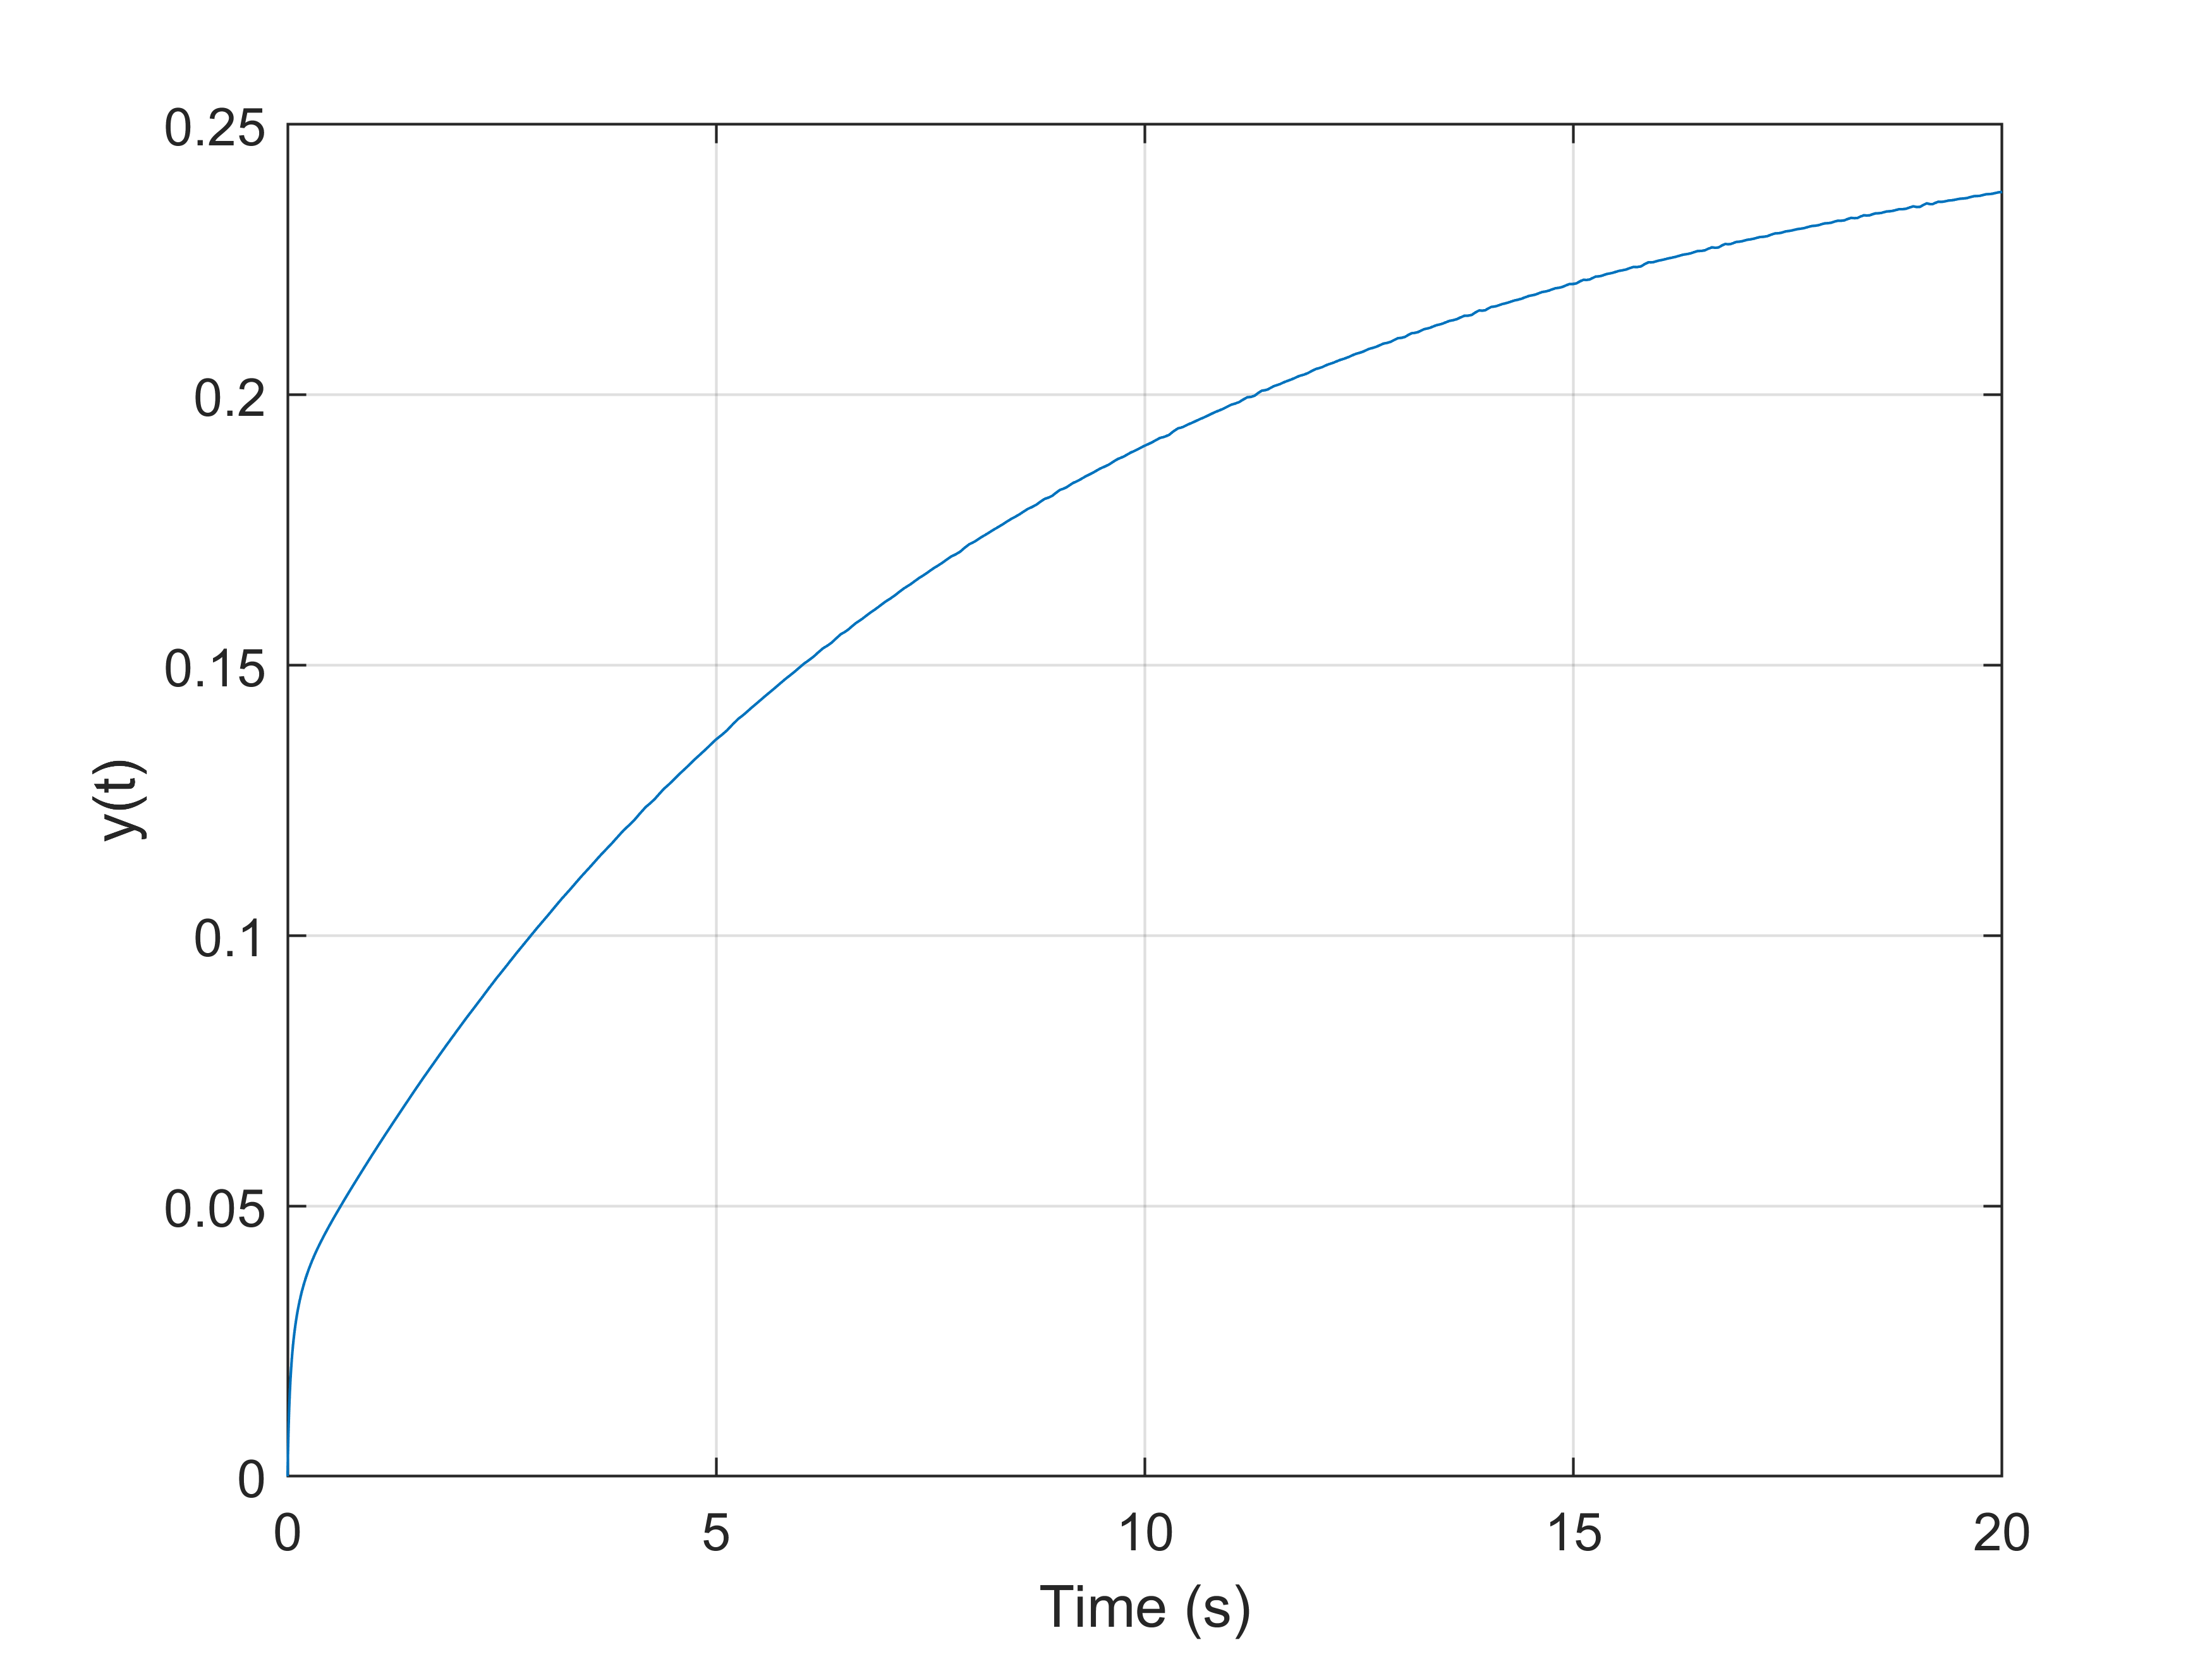
\includegraphics[width=0.6\textwidth]{figures/11_step_reference.png}
    \caption{Response of system to unit step reference signals}
    \label{fig:11_step}
\end{figure}

Figure \ref{fig:11_step} shows the step response of the closed loop system with the weights calculated above.
It's observed to be stable with a delayed response and reaches a final value of ~$0.26$ from the unit input.
The slow response is likely due to the smaller value of the slow network $z_1$ compared to the faster $w_2$.

\begin{figure}[H]
    \centering
    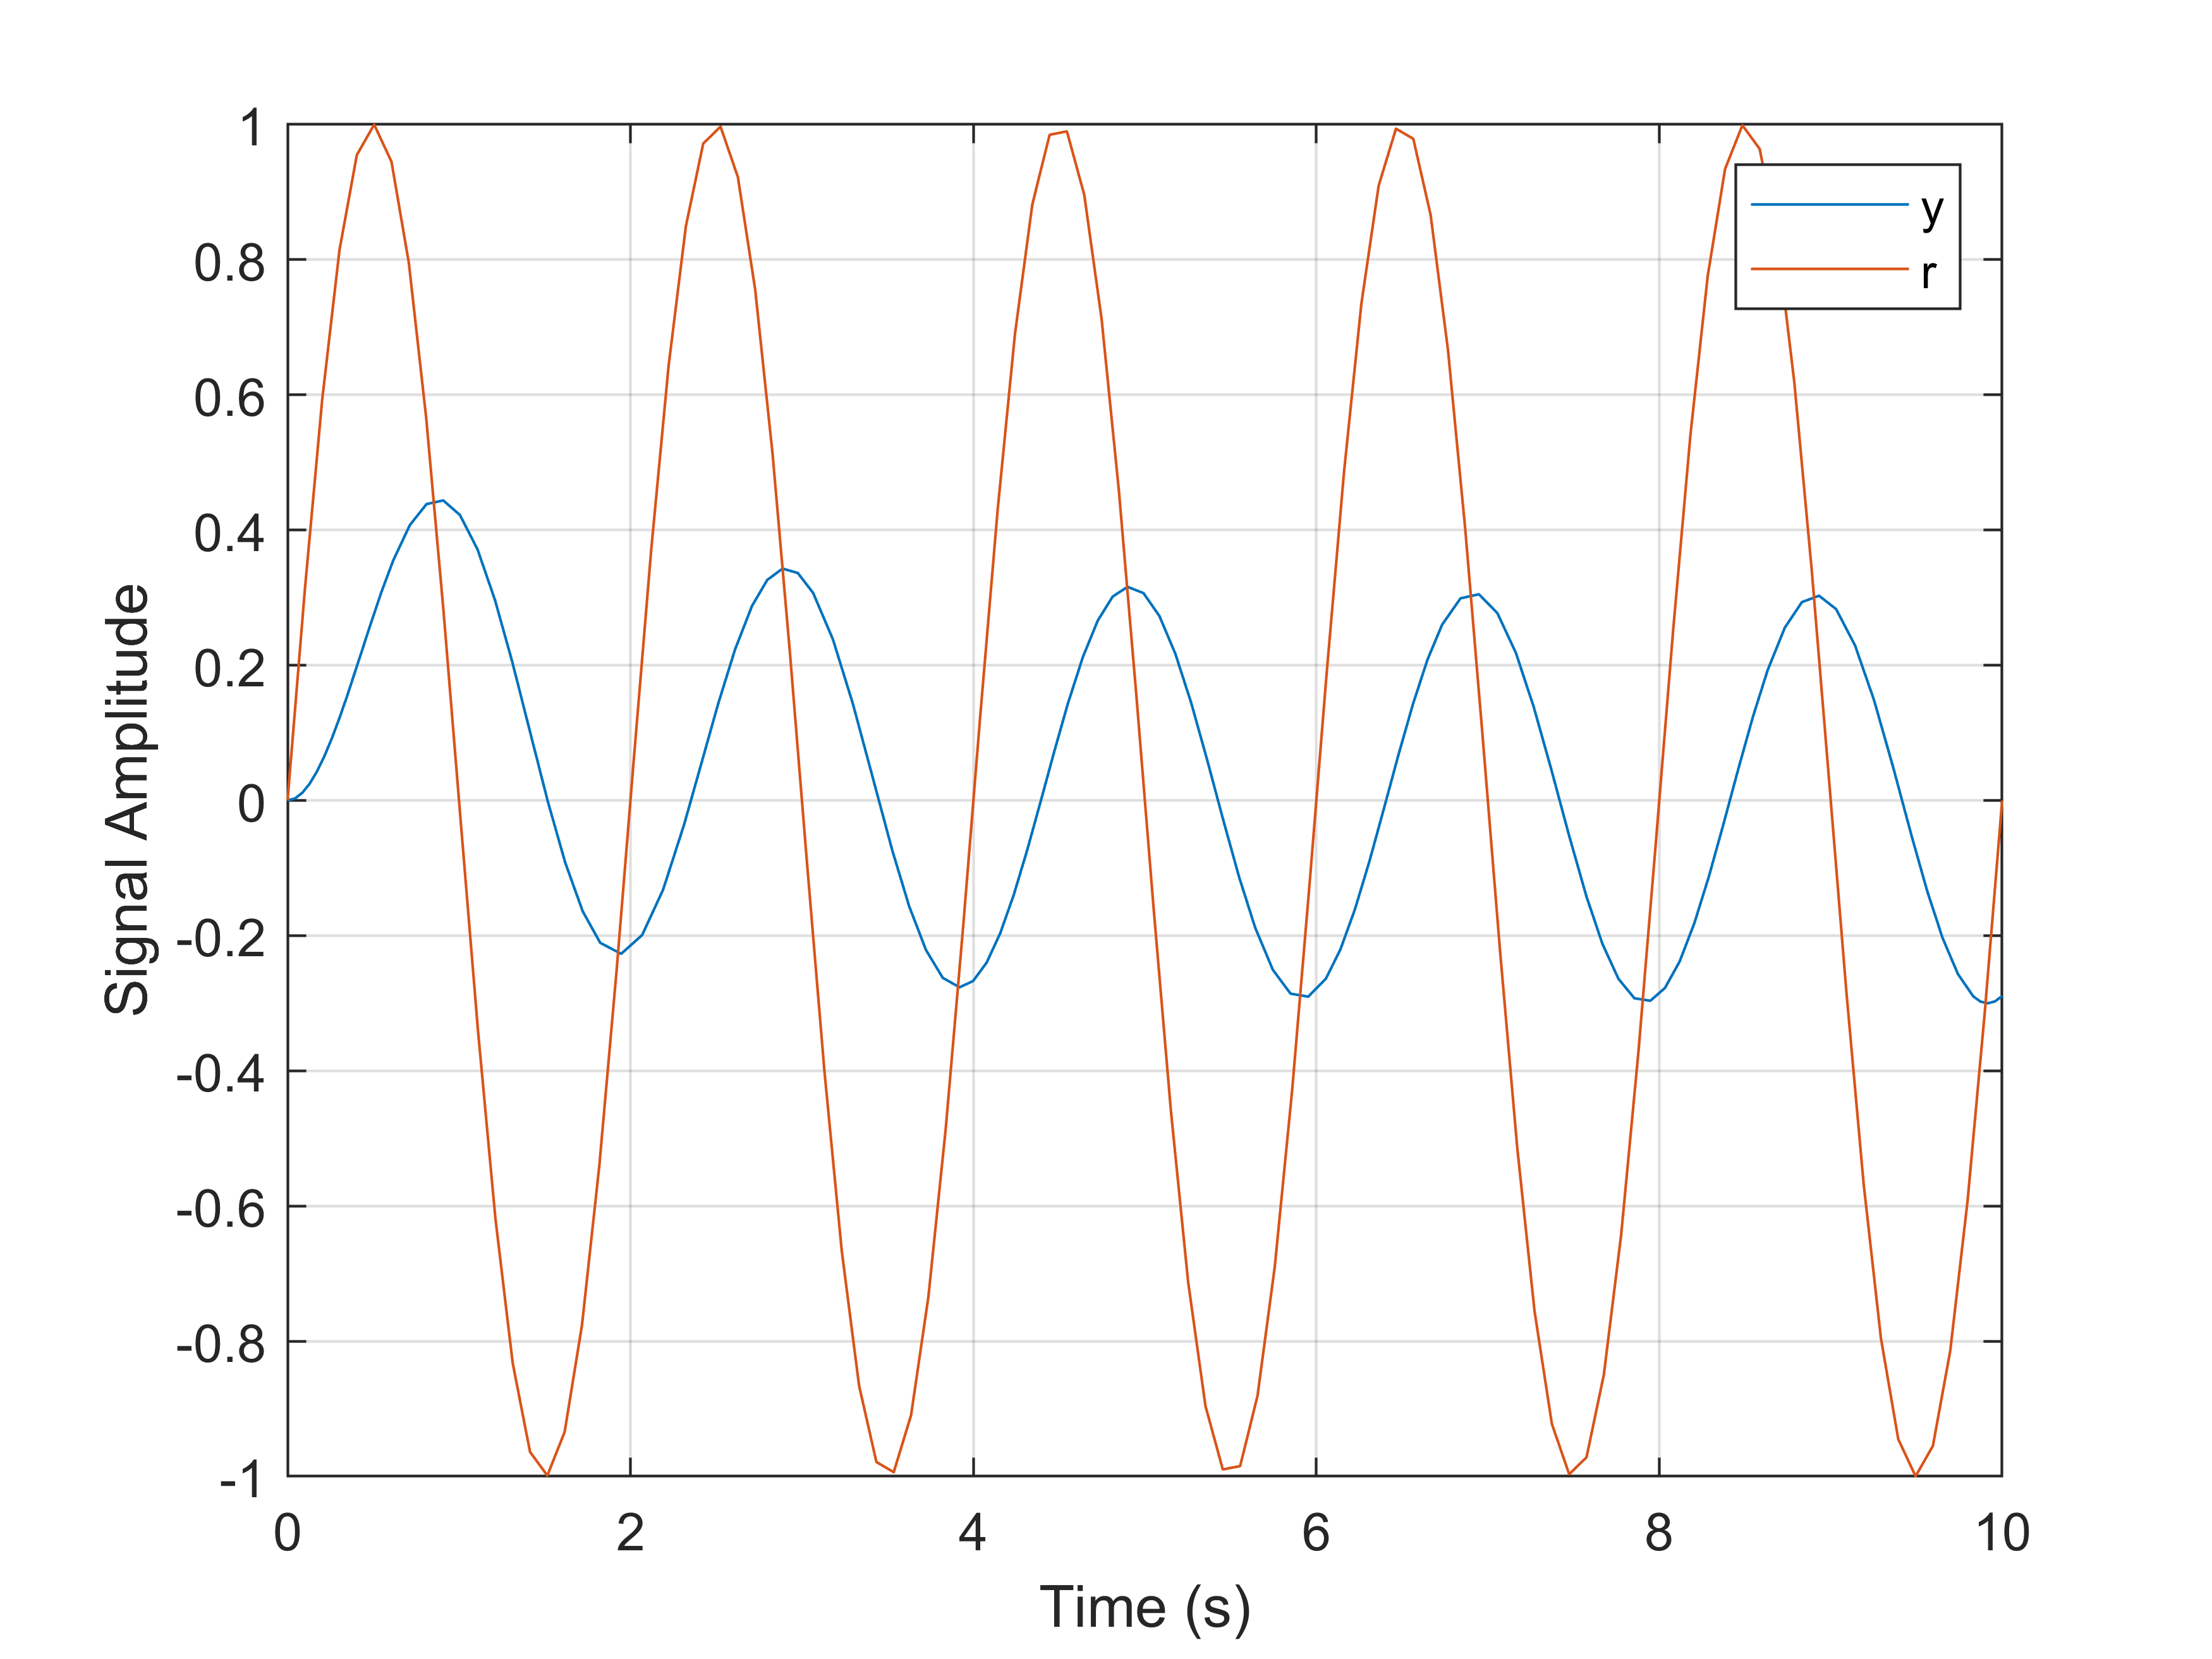
\includegraphics[width=0.6\textwidth]{figures/11_harmonic_reference.png}
    \caption{Harmonic reference signal and systems response}
    \label{fig:11_harmonic}
\end{figure}

The response in figure \ref{fig:11_harmonic} is for a unit sinusoidal reference signal with frequencies $0.5$ Hz and $1$ Hz.
Some phase lag is observed but is relatively small. The sinusoidal shape is not preserved which is expected from the nonlinearity of the system feedback.
The lower frequency seems to be warped more than the higher frequency, which is again likely due to the high weighting of the fast first order network $z_2$ compared to the slow $z_1$.

The dissipativity LMI in matrix form is given by
\begin{equation}    
\left[
\begin{array}{cc}
\partial f(x)^T P + P \partial f(x) + 2\lambda P & PB - \partial \varphi(x)^T \\
B^T P - \partial \varphi(x) & 0
\end{array}
\right] \leq 0.
\end{equation}

\subsection{Weights for autonomous nonlinear oscillator}
Neglecting the fast dynamics $w_2 = 0$, setting $w_3 = 25$ and taking $r = 0$ allows the
use of phase portrait on the reduced system to understand the variation with $w_1$.
\begin{equation}
    \dot{y} = -y + \varphi(w_1z_1 + 25y) \quad 0.1 \dot{z_1} = -z_1 + y
\end{equation}

\begin{figure}[H]
    \centering
    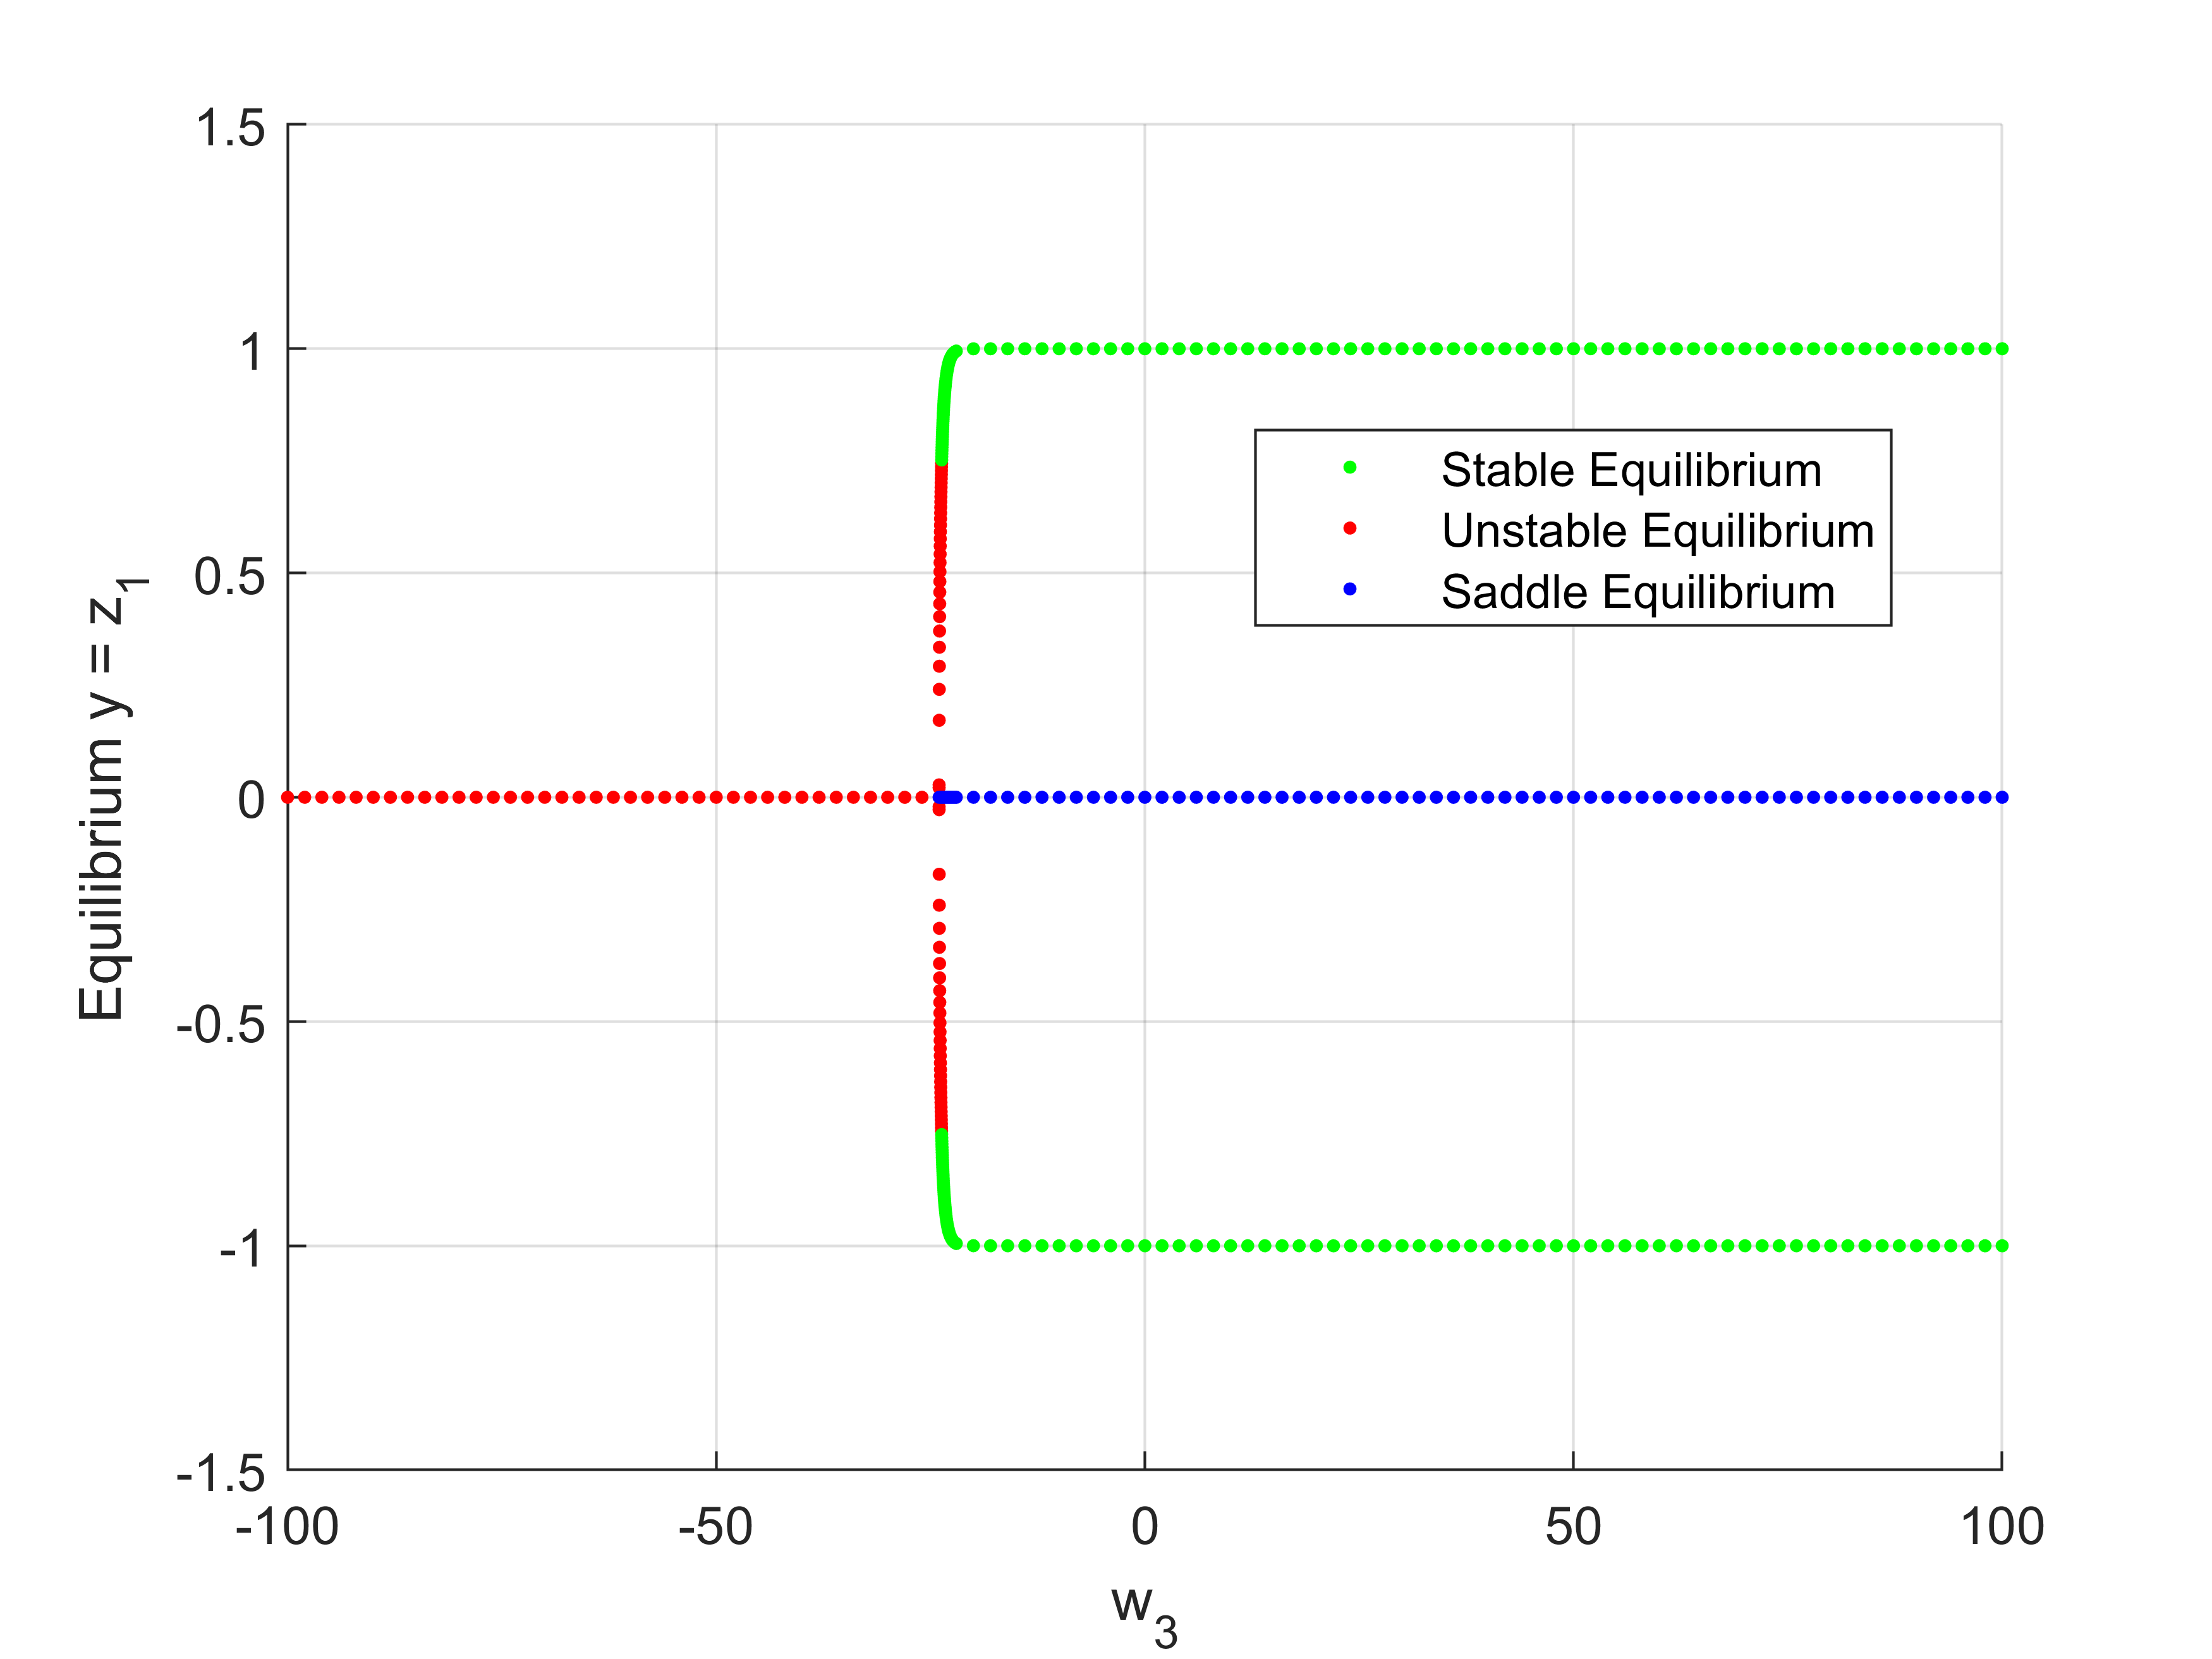
\includegraphics[width=0.6\textwidth]{figures/equilibria_bifurcation.png}
    \caption{Bifurcation of equilibria with varying $w_1$}
    \label{fig:equilibria}
\end{figure}

Figure \ref{fig:equilibria} shows the bifurcation of equilibria with varying $w_1$.
This occurs at a value of $w_1 = -24$ where the unstable equilibrium at $(0,0)$ becomes a saddle point (stability in one direction and instability in the other).
The direction of this can be seen by the phase portrait below in figure \ref{fig:phase_portrait_w100}.
Two stable equilibria form at $y = z_1 = \pm 1$ above this bound for $w_1$.


\begin{figure}[H]
    \centering
    \begin{subfigure}[b]{0.45\textwidth}
        \centering
        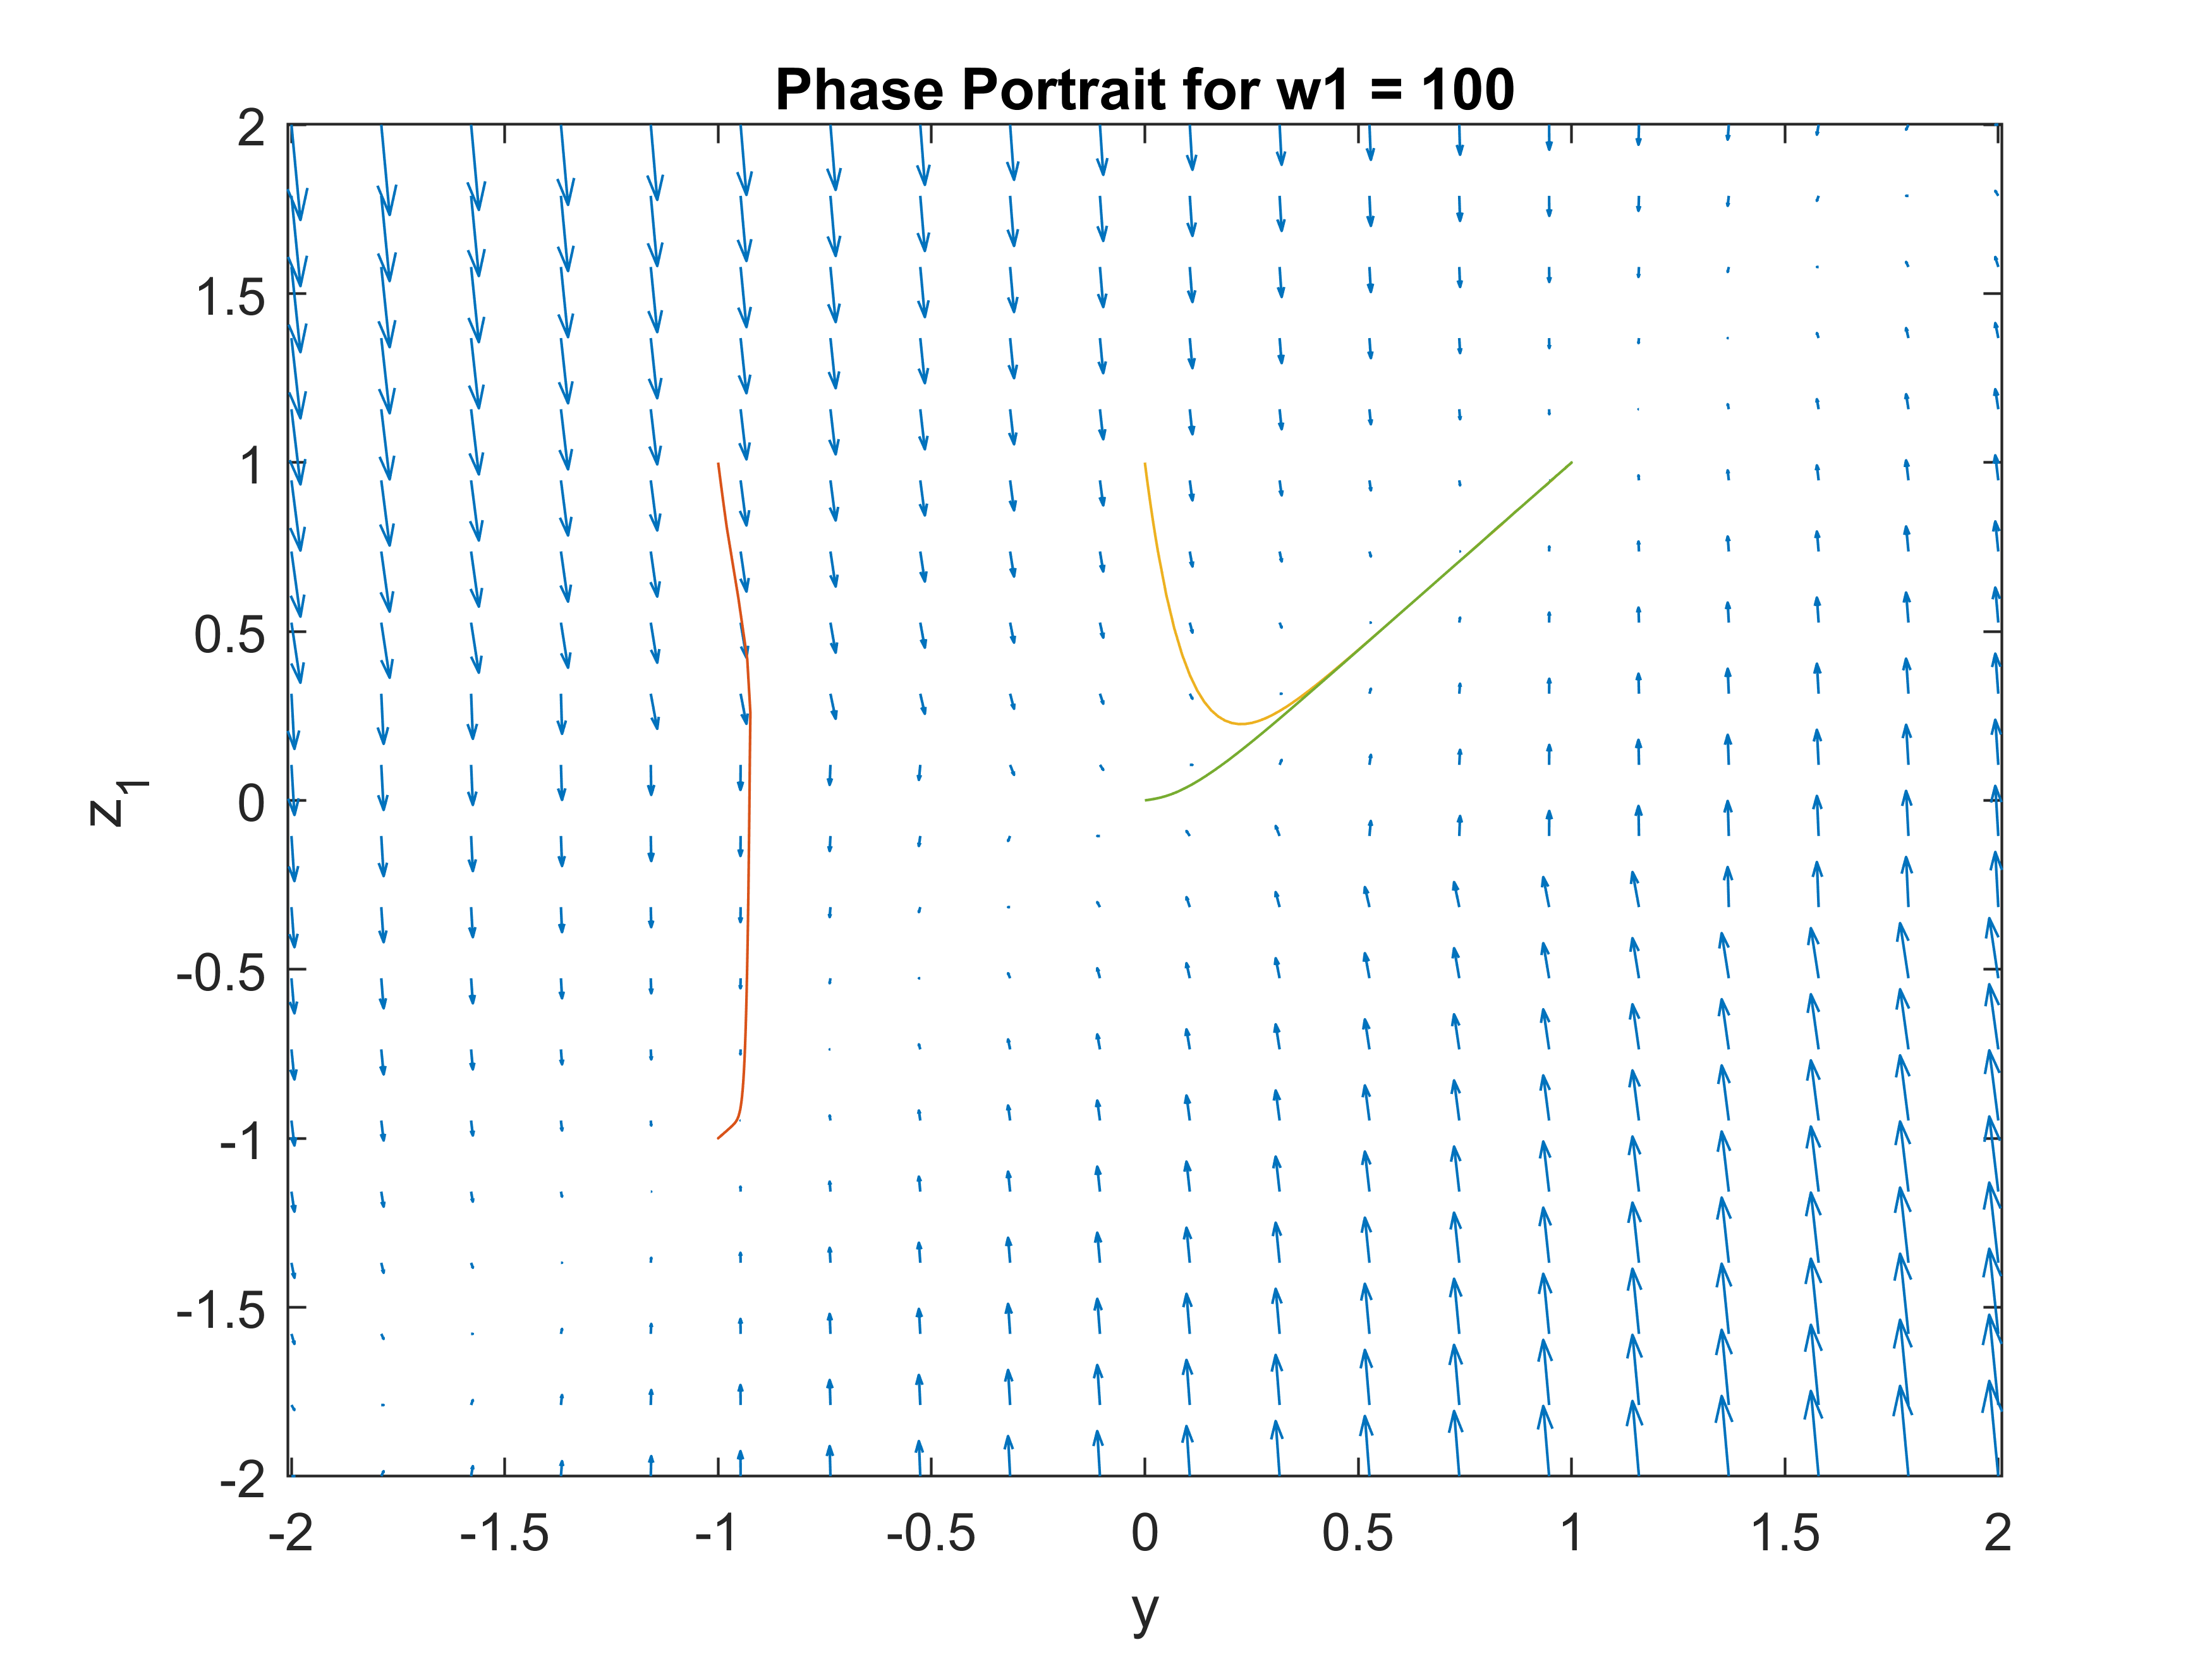
\includegraphics[width=\textwidth]{figures/oscillator_phase_portrait_w100.png}
        \caption{$w_1 = 100$}
        \label{fig:phase_portrait_w100}
    \end{subfigure}=
    \begin{subfigure}[b]{0.45\textwidth}
        \centering
        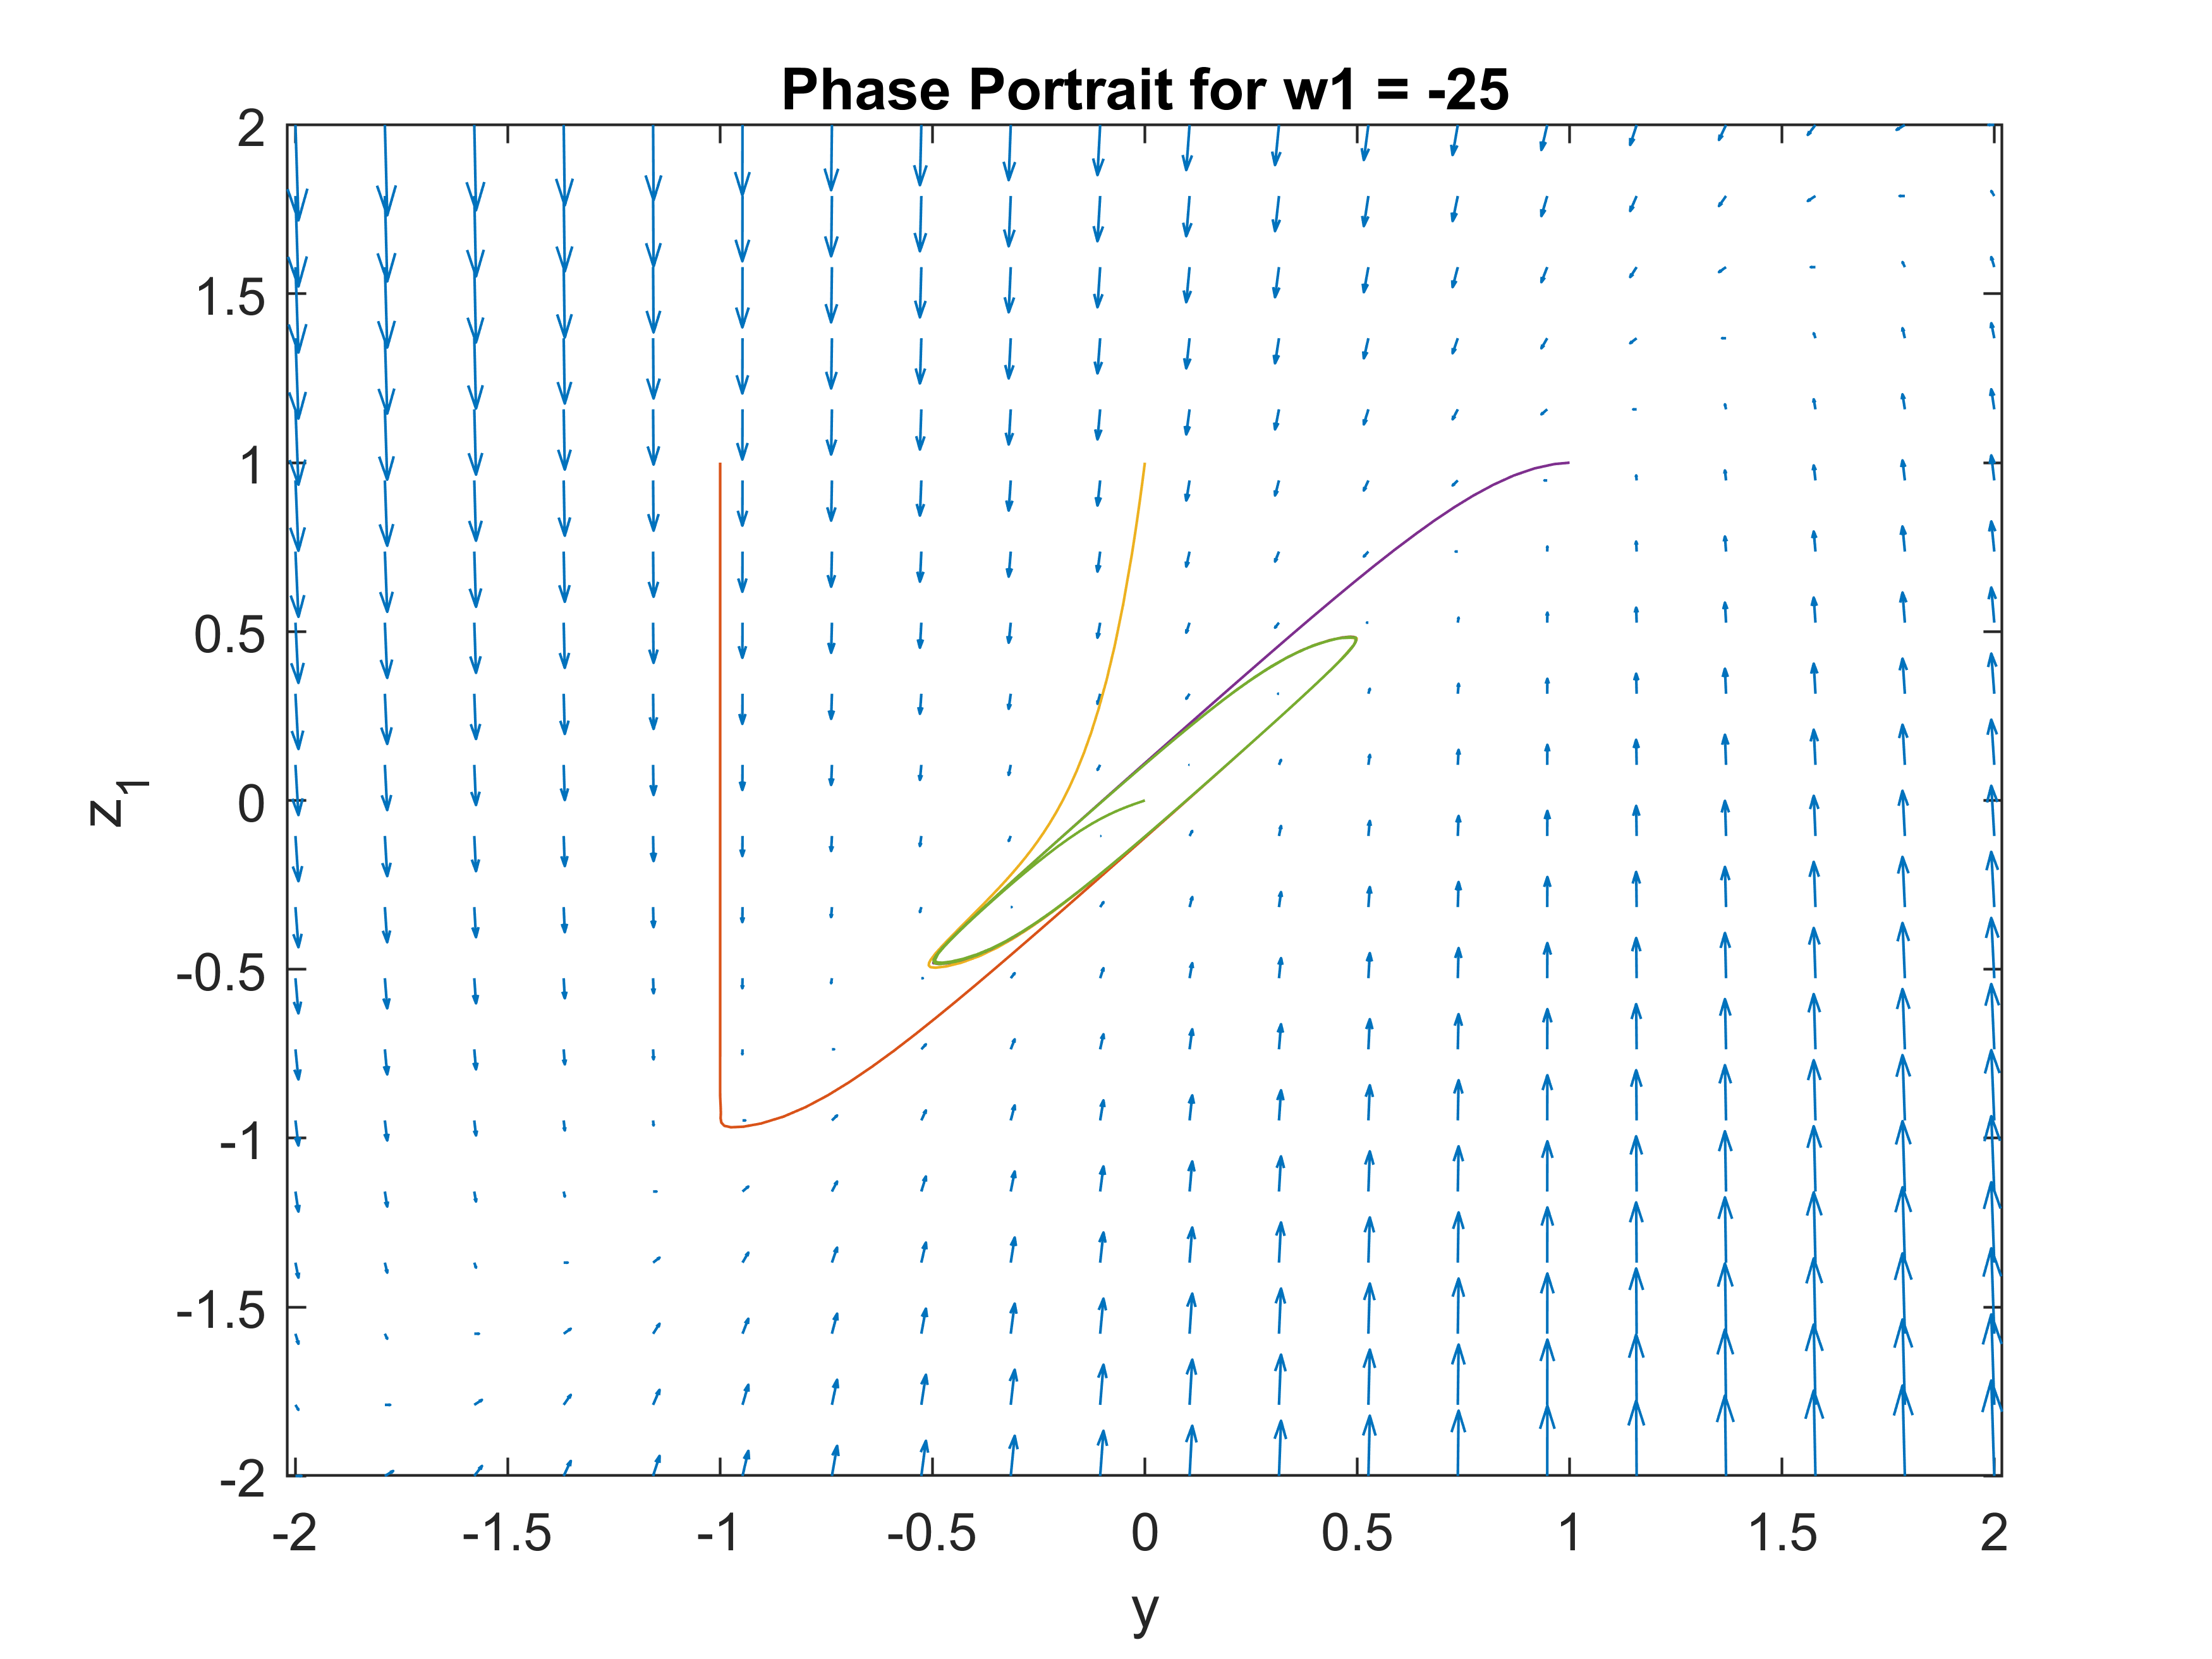
\includegraphics[width=\textwidth]{figures/oscillator_phase_portrait_w-25.png}
        \caption{$w_1 = -25$}
        \label{fig:phase_portrait_w25}
    \end{subfigure}
    \caption{Phase portrait of the autonomous nonlinear oscillator for varying $w_1$ to show the different equilibria}
\end{figure}

Figure \ref{fig:phase_portrait_w100} shows the phase portrait of the system with $w = [100, 0, 25]$.
The trajectories can be seen to converge towards the two stable equilibria which is expected from the bifurcation diagram \ref{fig:equilibria}.
For the system with $w = [-25, 0, 25]$ in figure \ref{fig:phase_portrait_w25} the system is seen to converge towards the unstable equilibrium at $(0,0)$.
However, for $w = [-25, 0, 25]$ the system is seen to be 2 dominant and oscillate around the unstable equilibrium.
State space trajectories also plotted, show initial conditions both inside and outside the oscillator path converge to the same cycle.


\subsection{Enforced 2-dominance and instability of 0 equilibrium}

Previously 2 dominance was observed from fixing $w_2 = 0$, $w_3 = 25$ and varying $w_1$.
This can be done more generally though the use of the LMI condition for 2-dominance.

\begin{align}
    \partial f Y + Y \partial f^T + 2\lambda Y + Z^T B_u^T + B_u Z + \varepsilon I &\leq 0 \\
    \partial f Y + Y \partial f^T + 2\lambda Y + \varepsilon I &\leq 0
\end{align}

This condition is required for oscillations however is not sufficient.
The last condition is instability of the 0 equilibrium which can be enforced by the LMI condition:

\begin{equation}
    Y \partial f(x)^T + \partial f(x) Y + Z^T B_u^T + B_u Z + \varepsilon I \leq 0
\end{equation}

To help the computation the $\varepsilon \geq 0$ is minimised.

\begin{figure}[H]
    \centering
    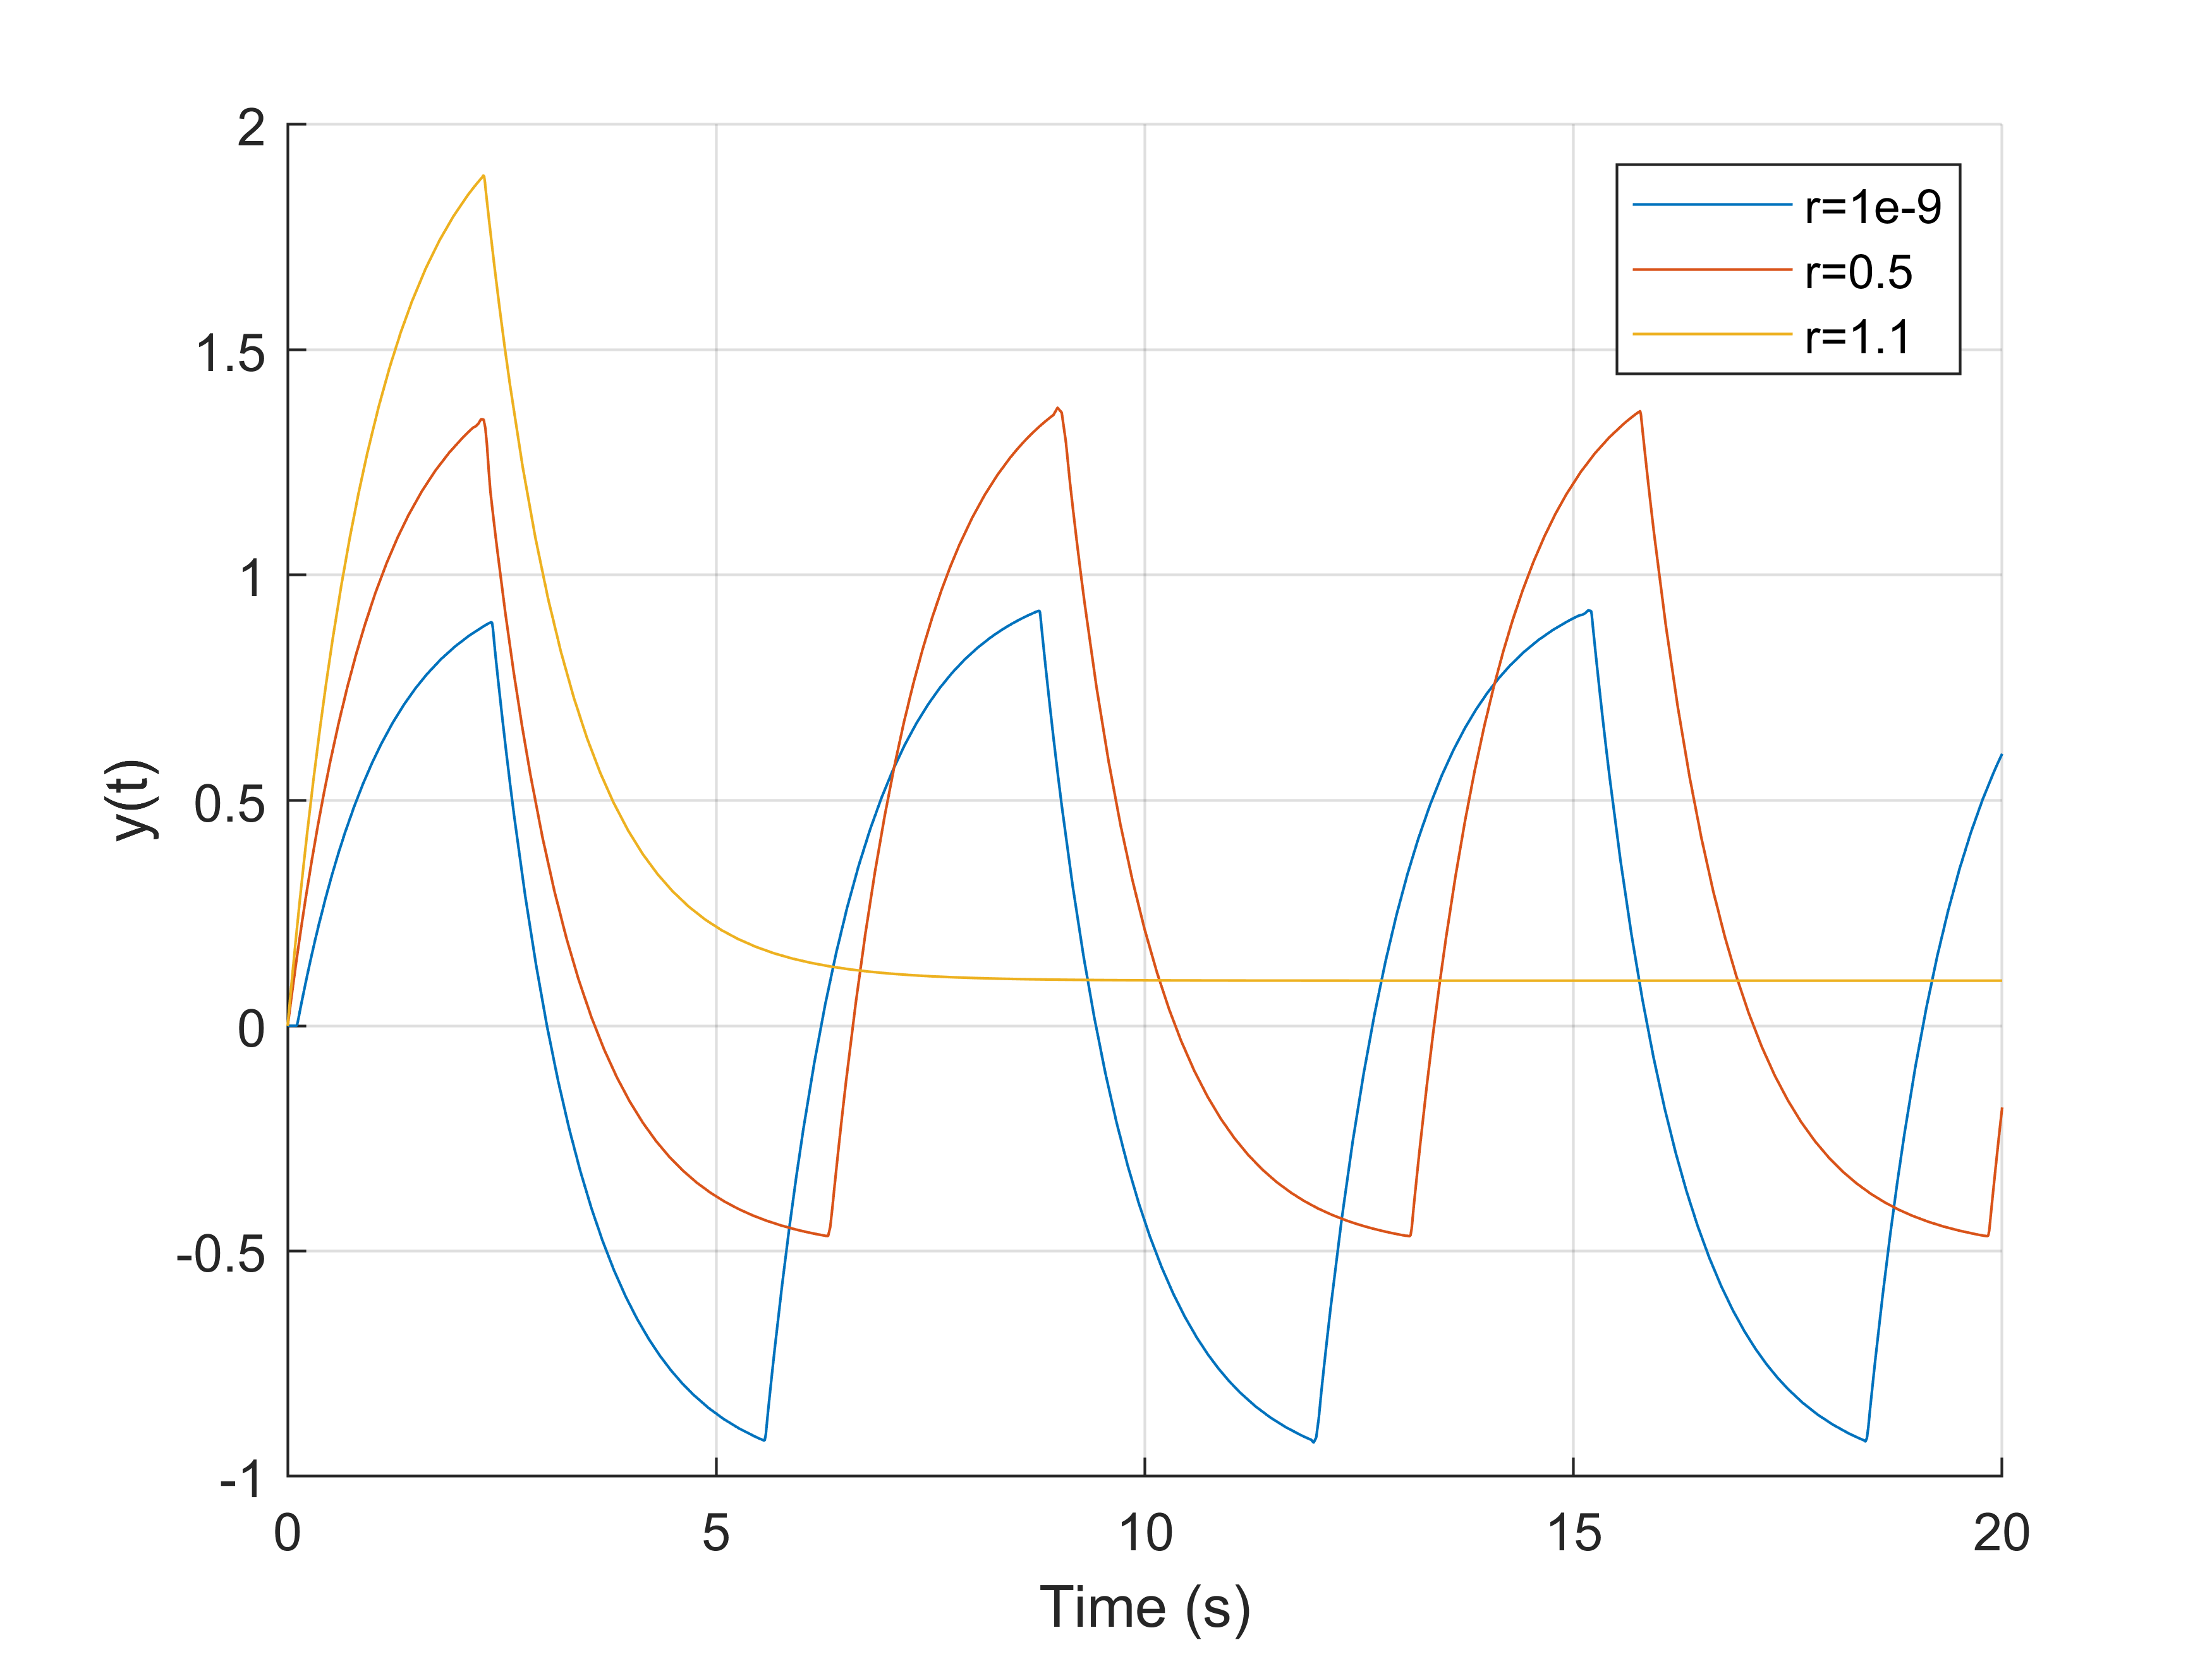
\includegraphics[width=0.6\textwidth]{figures/13_oscillator_responses.png}
    \caption{Responses of the oscillator to different constant reference inputs}
    \label{fig:13_responses}
\end{figure}

Figure \ref{fig:13_responses} shows the response of the system to different constant reference inputs.
It can be seen that a reference input of $r = 0$ produces no oscillation for the network started from rest, however a tiny reference input of $r=1e-9$ will cause the system to oscillate.
This is due to the unstable equilibrium at 0.
However its possible if a reference signal of above 1 is used the system will stop oscillating and converge to an equilibrium point.
This is the transition from 2-dominance to 1-dominance.

The open loop LTI system, G, can be used alongside the bounded non-linearity in the differential circle criterion for $p$-dominance.
$p$-dominance is satisfied if the Nyquist locus of $G(s-\lambda)$ does not intersect the disc with diameter $[-1/\alpha, -1/\beta]$ from the bounded non-linearity $\alpha \leq \partial tanh(x) < \beta$.
The sector condition of $\alpha=0$ and $\beta=1$ means the Nyquist locus of $G(s-\lambda)$ must not have a real part less than $-1$.
The value of $\lambda$ can be used to select the desired $p$ dominance, which a value of 20 is known to provide.
The region $\mathcal{R}_\text{2dom}$ is then defined as the set of parameters to satisfy this 2-dominance circle criterion condition.
The classic Nyquist criterion is also used to determine the subset of the system parameters, $\mathcal{R}_\text{inst}$, which are unstable, allowing oscillations to occur.

\begin{figure}[H]
    \centering
    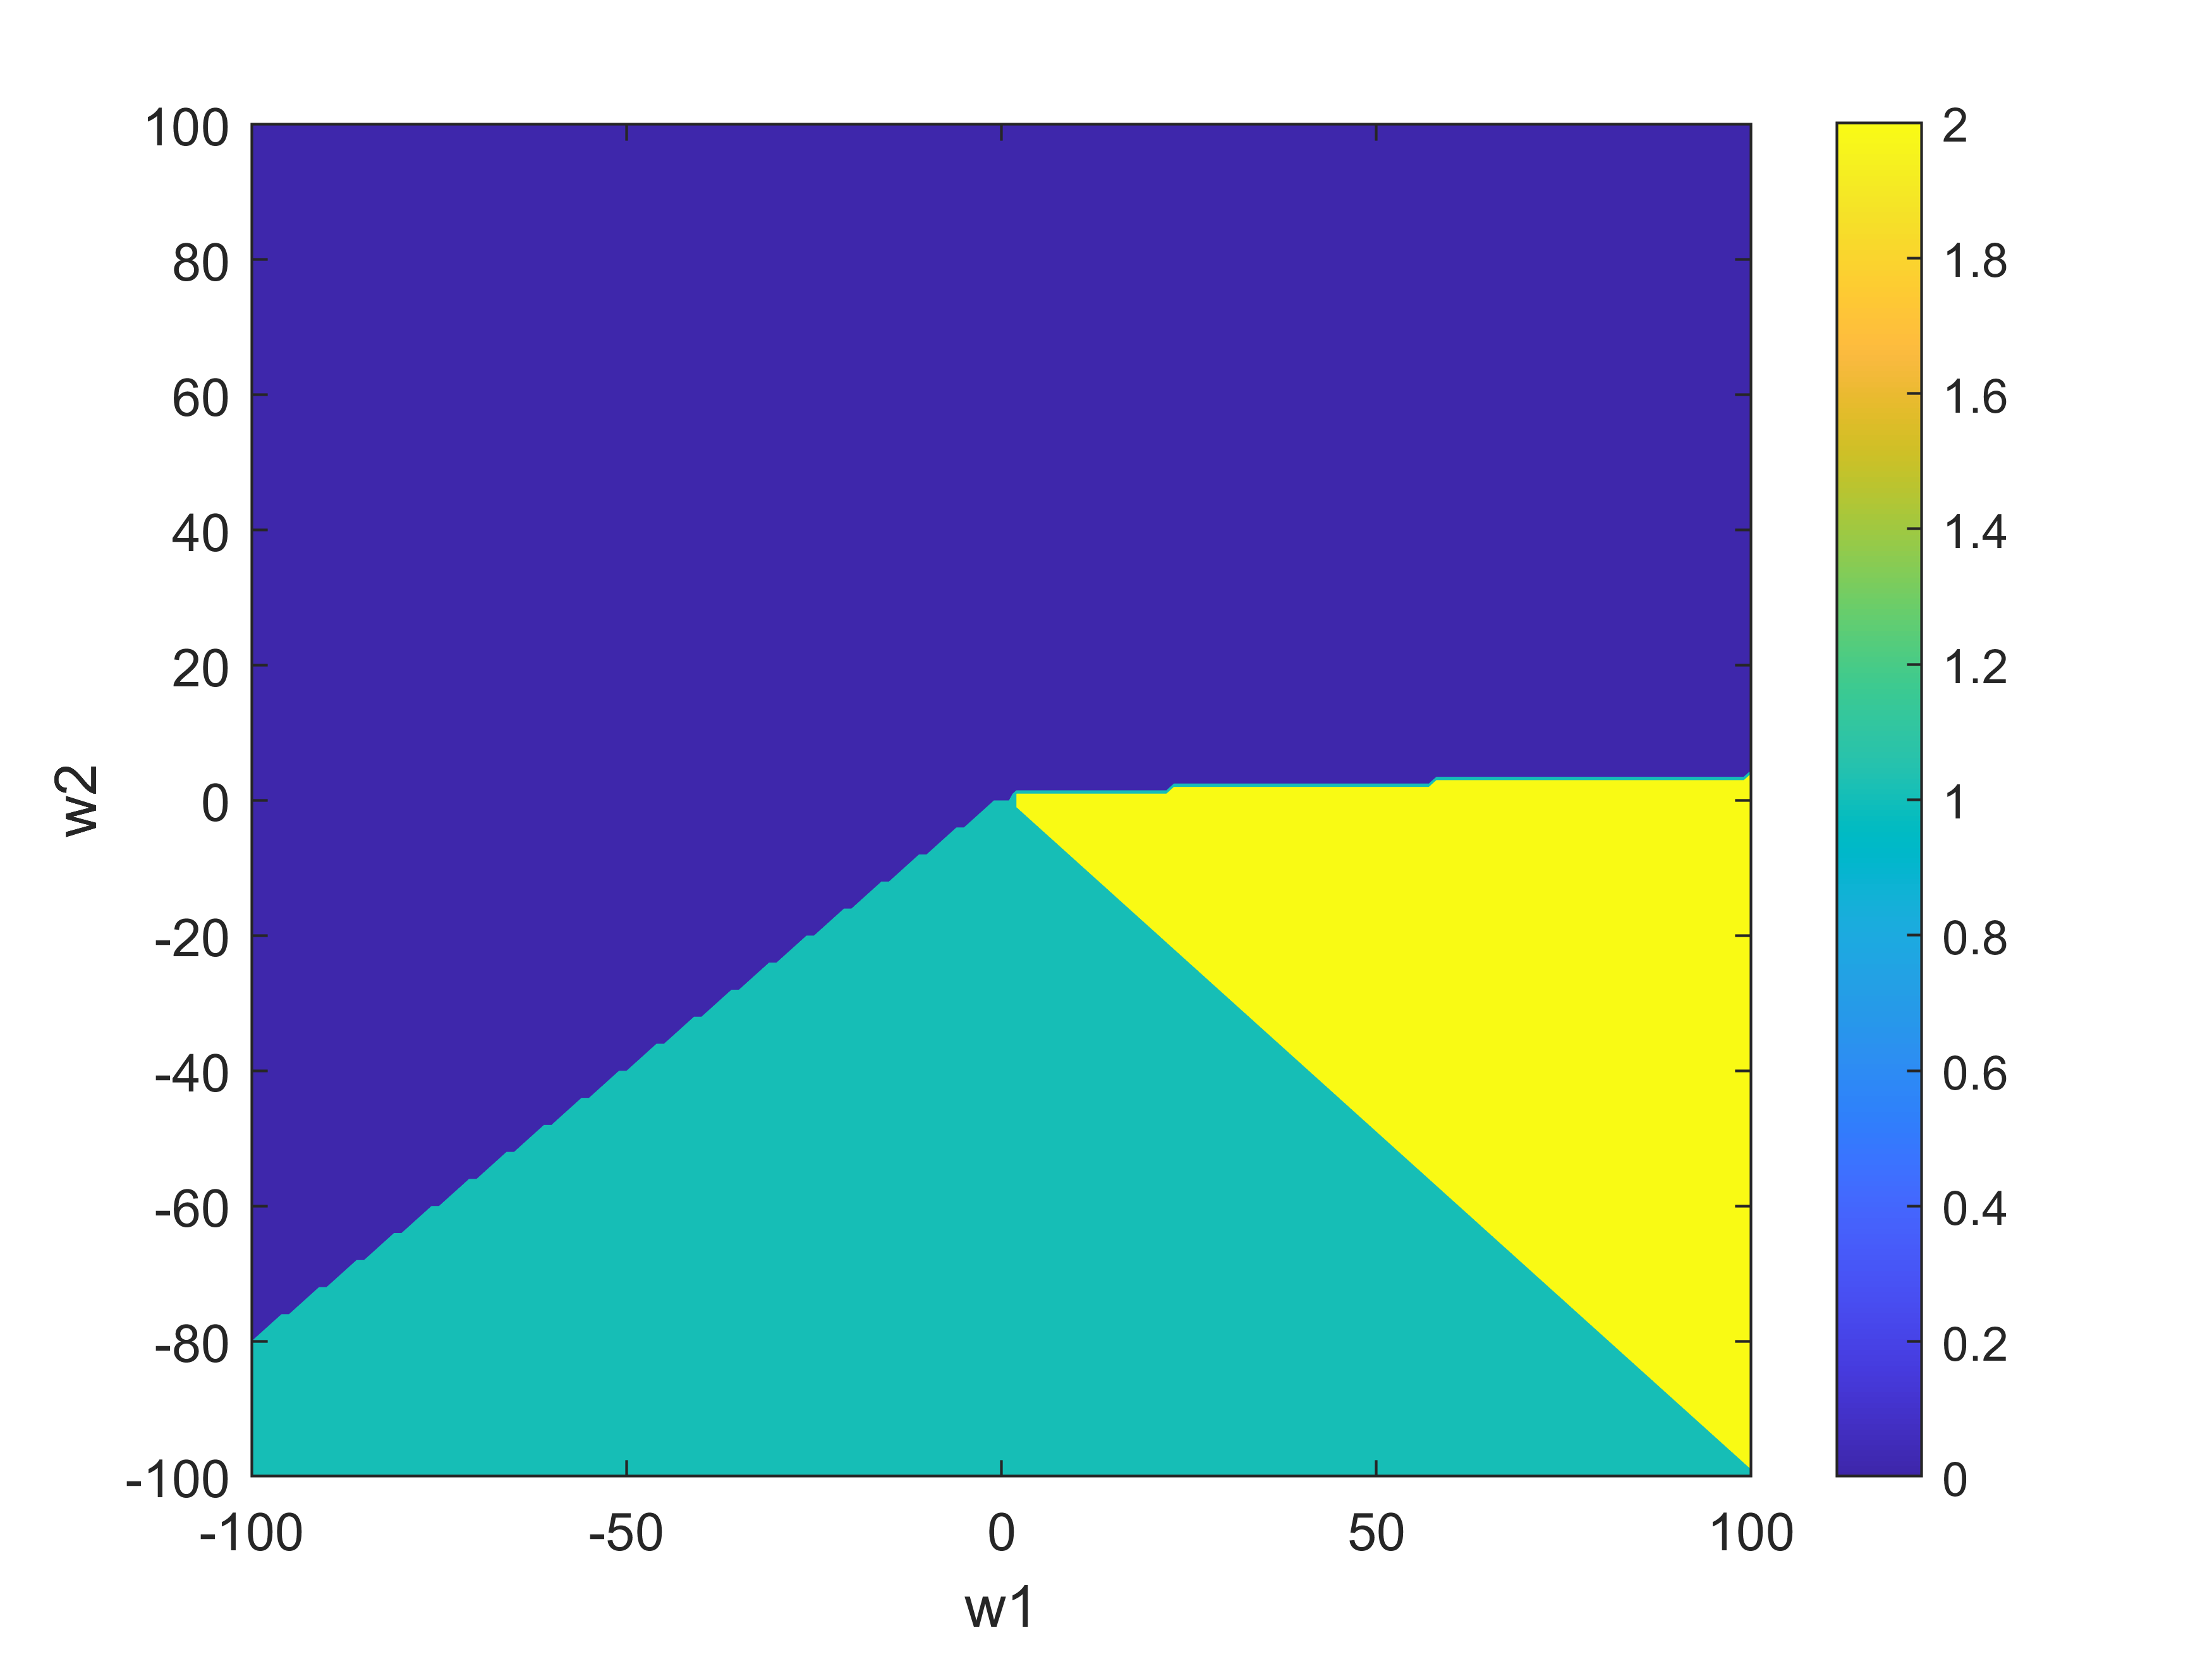
\includegraphics[width=0.6\textwidth]{figures/R2dom.png}
    \caption{Region $\mathcal{R}_\text{2dom}$ is shaded cyan and the subset $\mathcal{R}_\text{inst}$ is shaded yellow.}
    \label{fig:R2dom}
\end{figure}

$\mathcal{R}_\text{2dom}$ and subset $\mathcal{R}_\text{inst}$ are shown above in figure \ref{fig:R2dom}.
This is largely encompassed by $w_2 < 0$, however as before when $w_2 = 0$ 
For $w_2 = 0$ and $w_1 = 24$ the system enters a very thin band inside $\mathcal{R}_\text{2dom}$ but not $\mathcal{R}_\text{inst}$,
which corresponds to the narrow range of $w_1$ values over which the equilibria bifurcate in figure \ref{fig:equilibria}.
However, this occurs close to $w_1 = -24$ which is identical because the circle criterion has been performed on $y \to -z$.
For higher $w_1$ seen in figure \ref{fig:R2dom} or lower $w_1$ in figure \ref{fig:equilibria} the system is 2-dominant and oscillates around the unstable equilibrium at $(0,0)$.

\subsection{Application of oscillator to small robotic insect}

The oscillator is used to drive a 
\begin{equation}
    m\ddot{x} + c_v \dot{x} + c_p x = u_m \quad \text{and} \quad y_m = 30x + \dot{x}
\end{equation}
Where $m = 0.001$, $c_v = 0.1$, $c_p = 2 \pm 0.1$.

\subsubsection{Excess output passivity of insect wing model}

The linear matrix inequality for p-passivity with excess/shortage $(\alpha, \beta)$ and rate $\lambda \geq0$ is given by
\begin{equation}
    \left[
    \begin{array}{cc}
    \partial f(x)^T P + P \partial f(x) + 2 \lambda P - \alpha \partial \varphi(x)^T \partial \varphi(x) + \varepsilon I & P B - \partial \varphi(x)^T \\
    B^T P - \partial \varphi(x) & -\beta I
    \end{array}
    \right] \leq 0. \quad \text{with} \quad \varepsilon > 0
\end{equation}
The input passivity, $\beta$, is set to 0, and the output passivity $\alpha$ as a CVX variable to be solved for with the constraint that its in excess $\alpha > 0$.
This gives the solution for $\alpha = 62.61$ showing that the system has excess output passivity.

\subsubsection{Designing w for equivalent input passivity shortage}

\begin{equation}
\left[
\begin{array}{ccc}
Y \partial f(x)^T + \partial f(x) Y + 2\lambda Y + Z^T \partial \varphi^T + \partial \varphi Z + \varepsilon I & B_w - Y C^T & Y C^T \\
B_w^T - C Y & -(D_w + D_w^T) - \beta I & D_w^T \\
C Y & D_w & \frac{1}{\alpha} I
\end{array}
\right] < 0 \label{eq:mega_lmi}
\end{equation}

The oscillator is designed to match its shortage in input passivity, $\beta_o$, to the wing models excess output passivity, $\alpha_w$.
The output passivity of the oscillator, $\alpha_o$ is set to 0 which means that the 3rd row and column of \ref{eq:mega_lmi} can be removed.
As before, the convex hull of two LMI's from the bounded nonlinearity are used.
Again, the instability of the 0 equilibrium is also enforced to guarantee oscillations.
The weights were then found as \texttt{[-117.2404,   31.7156,   39.5764]}.

\subsubsection{Excess and shortage of passivity in the closed loop }

\begin{figure}[H]
    \centering
    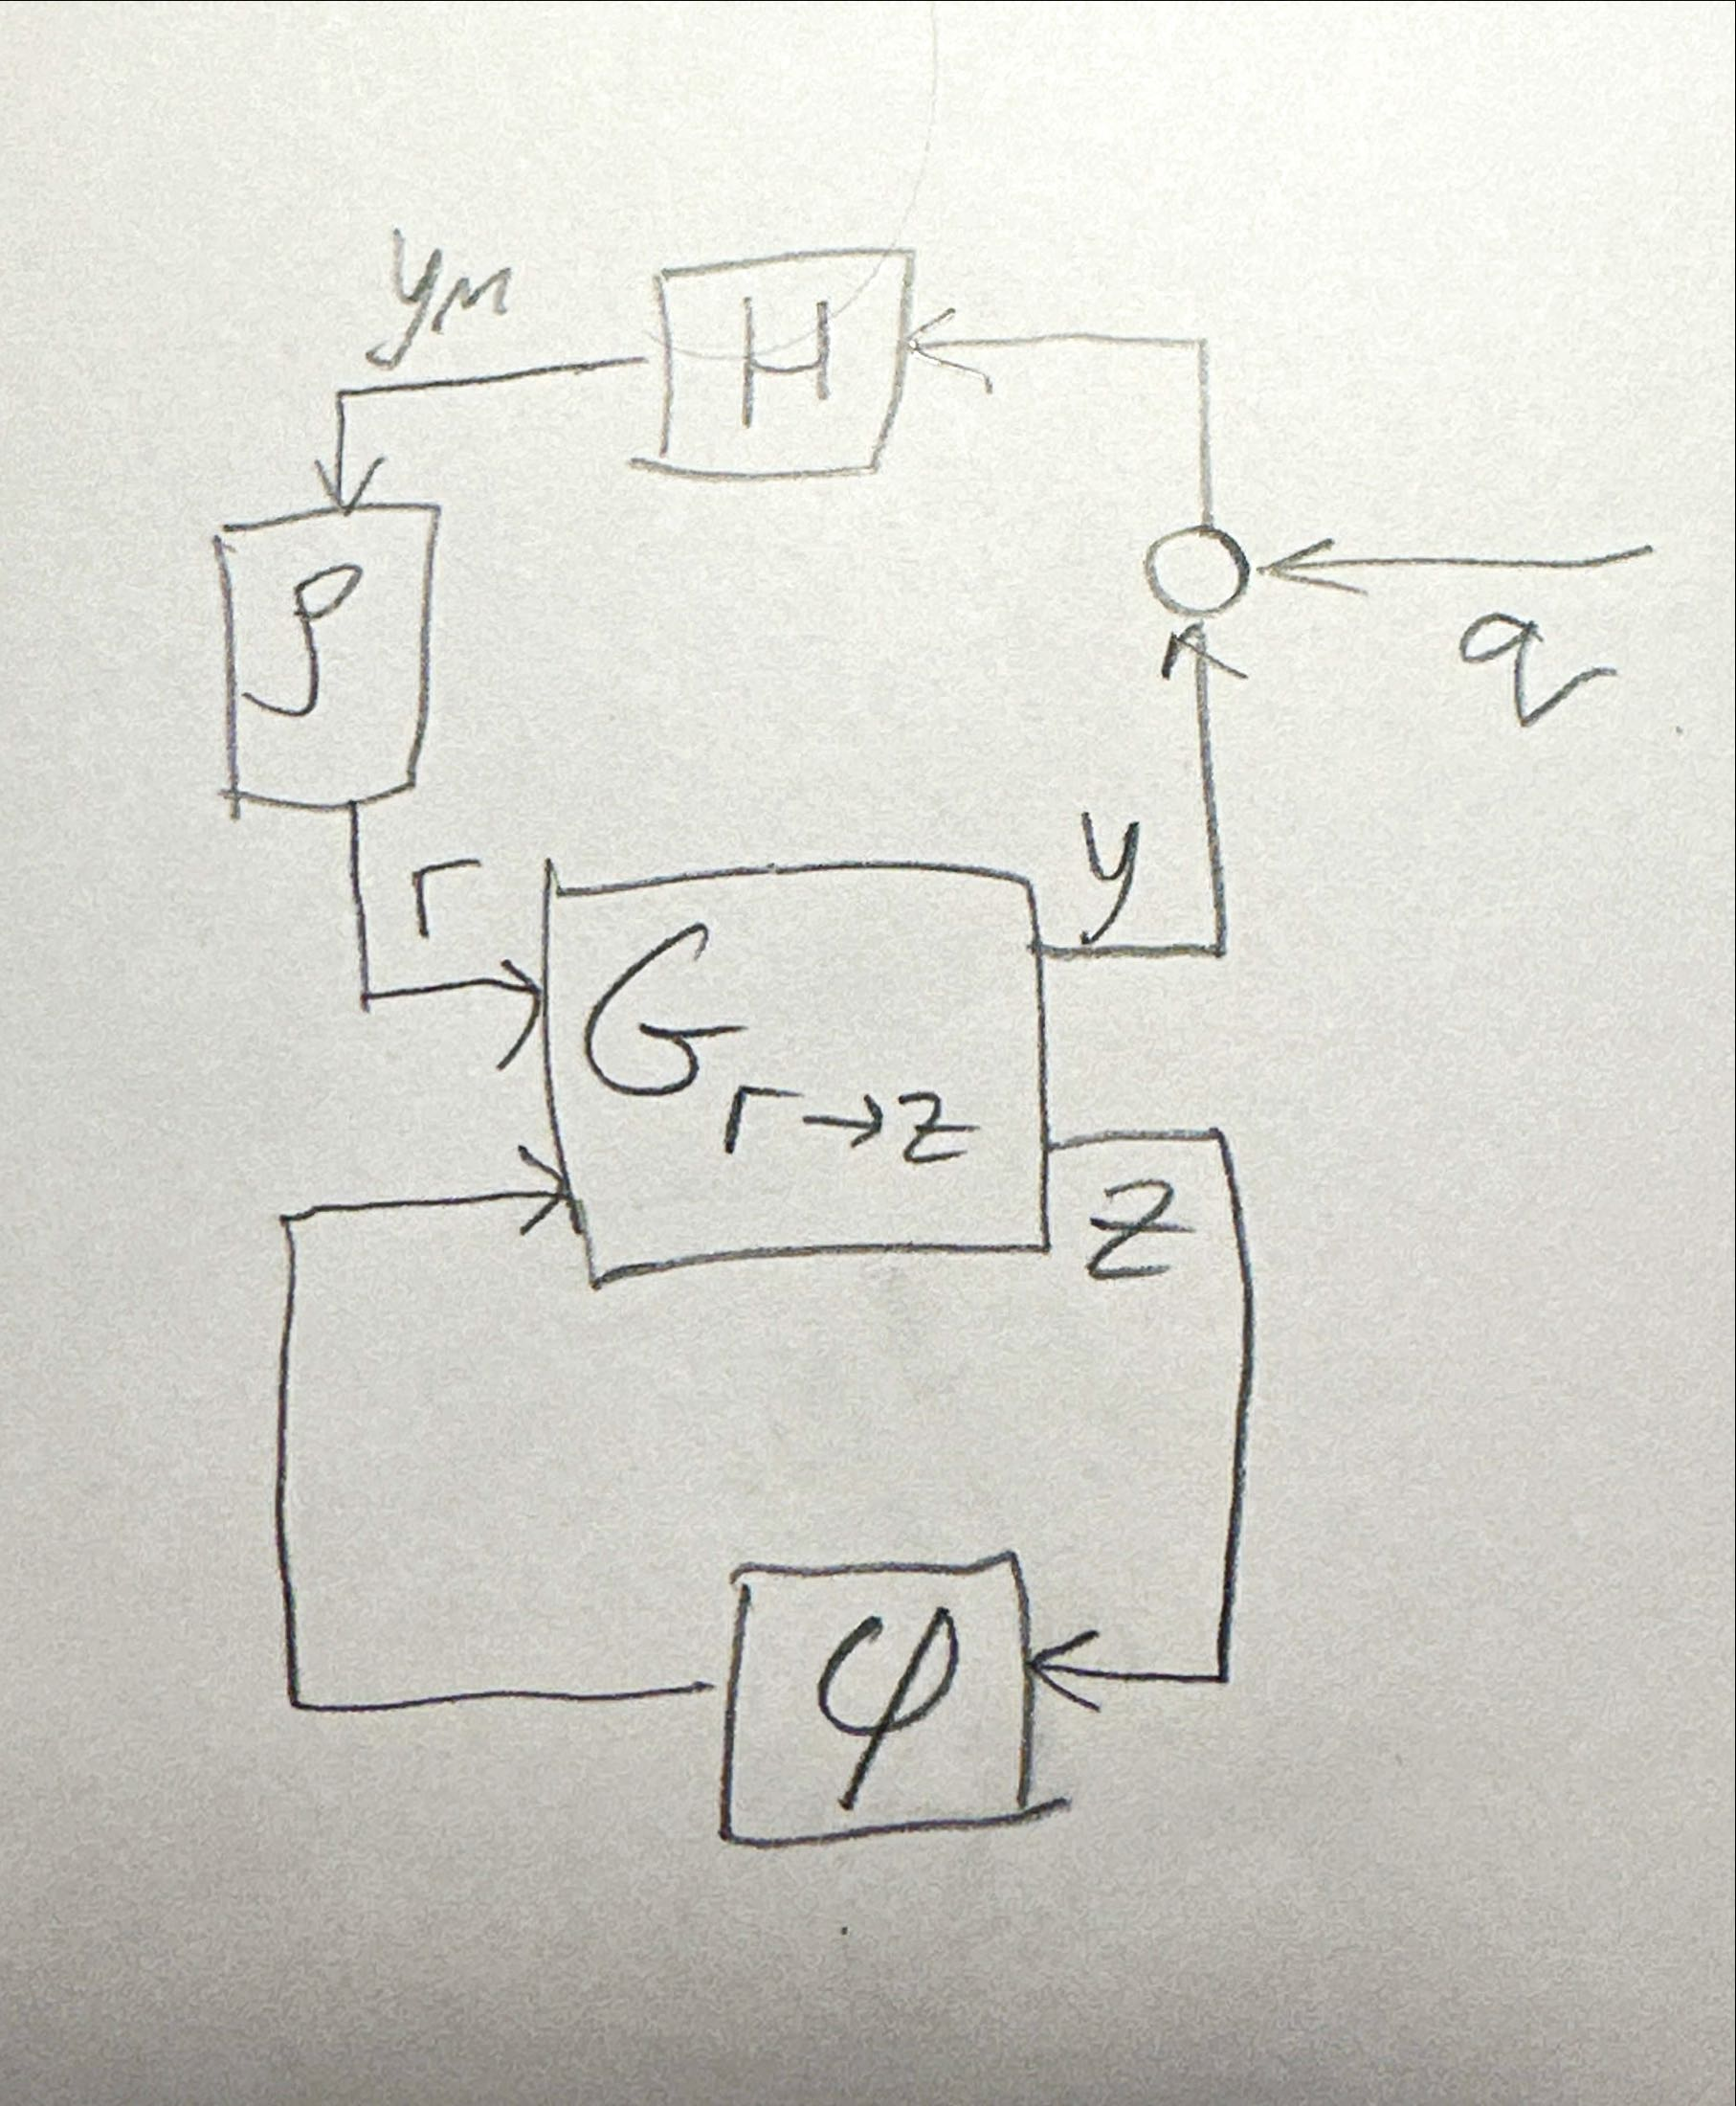
\includegraphics[width=0.2\textwidth]{figures/excess_shortage.jpg}
    \caption{Feedback interconnection of the insect wing model and oscillator}  
    \label{fig:excess_shortage}
\end{figure}

The passivity theorem with excess/shortage of passivity states that for the systems $G$ and $\rho H$ in figure \ref{fig:excess_shortage} with feedback interconnections:
\begin{equation}
    r = \rho y_m = H u_m \quad \text{and} \quad u_m = y + q
\end{equation}
Then the closed loop is $(p_G + p_{\rho H})$-dominant with common rate $\lambda$ if $\alpha_G + \beta_{\rho H} \leq 0$ and $\alpha_{\rho H} + \beta_G \leq 0$.
Where $G$ is $p_G$-passive with shortage/excess $(\alpha_G, \beta_G)$ and $\rho H$ is $p_{\rho H}$-passive with shortage/excess $(\alpha_{\rho H}, \beta_{\rho H})$.

The range of $\rho$ at which the requirement $\alpha_{\rho H} + \beta_G \leq 0$ is satisfied was not found due to time constraints.
The method for finding this would be to manually check different values of $\rho$ in the LMIs \ref{fig:determining_excess_output_passivity_lmi} and \ref{fig:equivalent_shortage_input_passivity_lmi}.

\subsection{Periodic input driven contractive network}

The input signal $r$ of the network designed in i) was designed such that the output resembled the oscillator network in iii).
The matched harmonic input had amplitude 3, frequency of 0.6440 rad/s and phase of 0.5 rad and phase difference of $\pi/4$.

\begin{figure}[H]
    \centering
    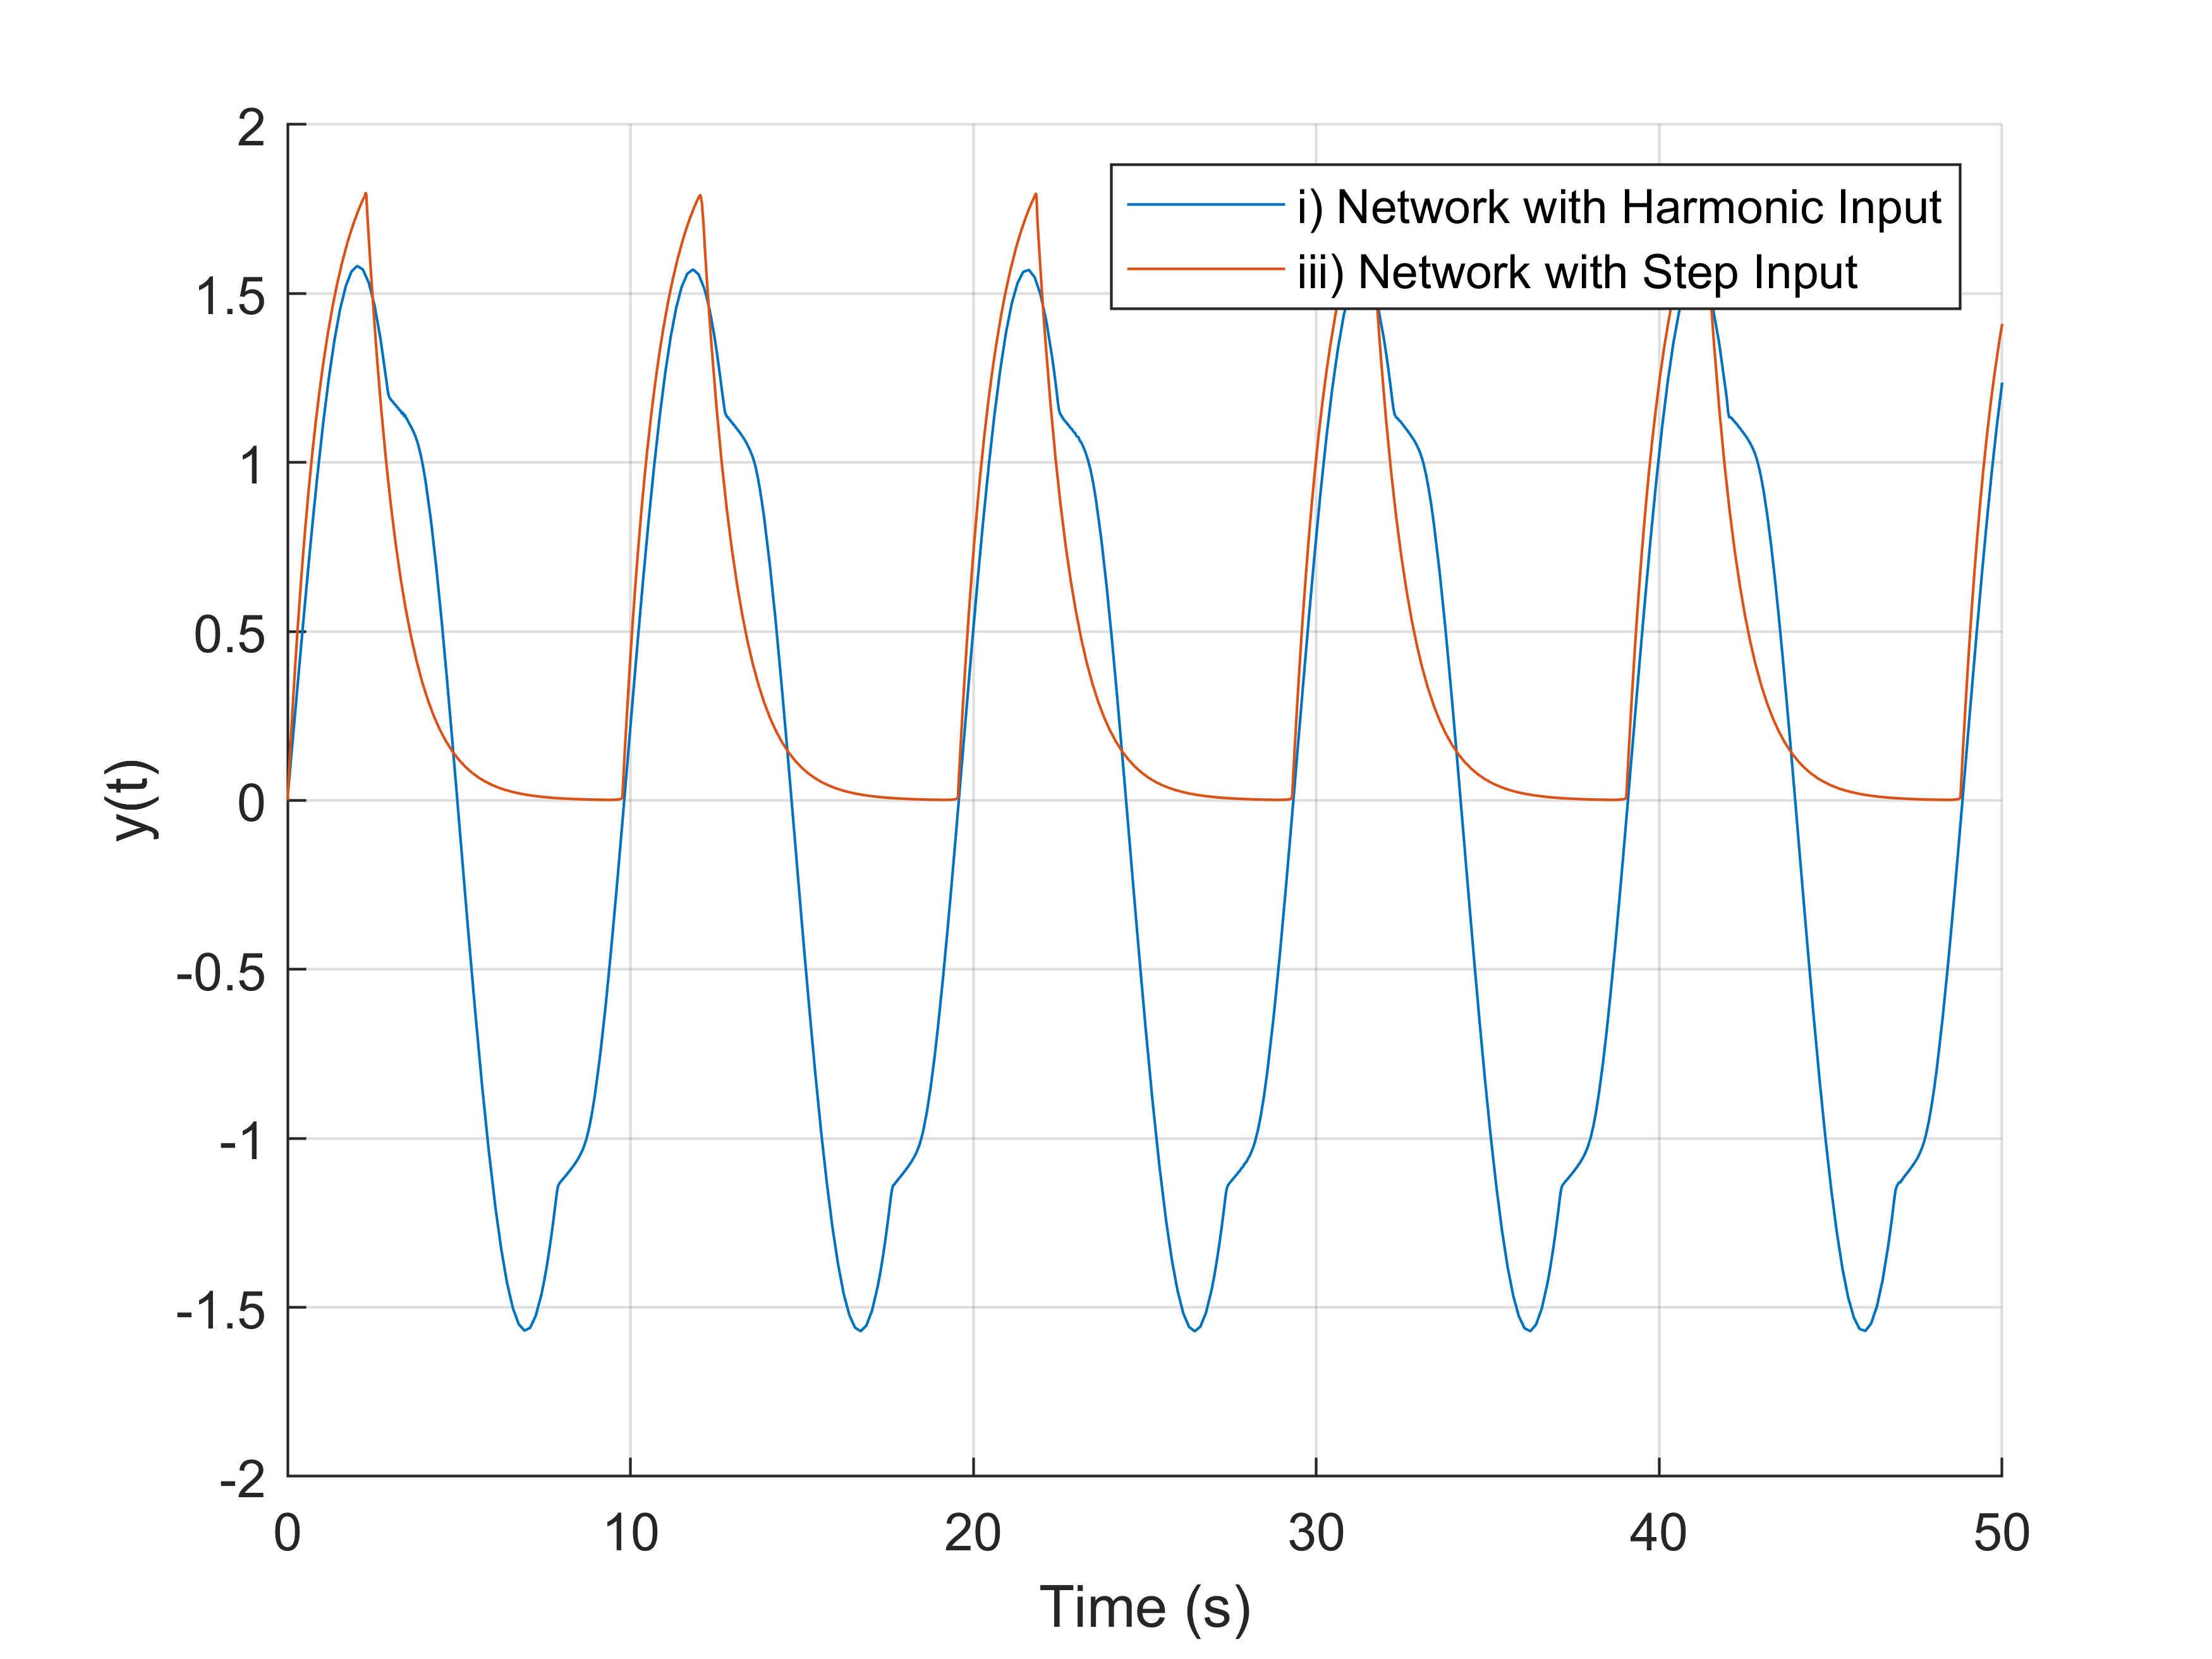
\includegraphics[width=0.2\textwidth]{figures/15_matched.png}
    \caption{Matched harmonic input to the oscillator network}  
    \label{fig:matched_harmonic_input}
\end{figure}

Figure \ref{fig:matched_harmonic_input} shows the matched harmonic input to the oscillator network.
It can be seen that half the cycle matches quite closely but the oscillator has an offset from 0 which is not replicated in the output from harmonic input.
% pros and cons


\section{Pharmacokinetics and drug dosage}

The drug concentration in two compartments are modelled by coupled differential equations:
\begin{align}
    V_1 \dot{c}_1 &= - \rho_1(c_1) - \alpha_{12}c_1 + w_1 \\
    V_2 \dot{c}_2 &= - \rho_2(c_2) - \alpha_{21}c_2 + w_2
\end{align}

$w_i$ are exogenous inputs, $\rho_i()$ are degradation functions which each obey the incremental sector condition
\begin{equation}
    \lambda_i \leq \frac{\rho_i(x_2) - \rho_i(x_1)}{x_2 - x_1} \leq \mu_i \quad \forall x_1, x_2 \in \mathbb{R} \quad \text{ where } \quad 0 < \lambda_i \leq \mu_i
\end{equation}
Drug concentration in the body is modelled using the positive feedback interconnection of the two compartments given by the equations:
\begin{align}
    w_1 &= \alpha_{21} c_2 + u \\
    w_2 &= \alpha_{12} c_1
\end{align}
where $u$ is an external drug dosage.
\subsection{Scaled relative graphs}

\subsubsection{Single compartment}

For compartment $i$ the incremental form is given by

\begin{equation}
    w_i = V_i \dot{c}_i + \alpha_{i,3-i} c_i + \rho_i(c_i)
\end{equation}

This can be decomposed into a linear part $L(c_1)$ and a nonlinear part $N(c_1)$:
The Scaled Relative Graph (SRG) from $w_1$ to $c_1$ is then derived by

\begin{align}
    w_1 &\in (L + N)(c_1) \\
    \implies c_1 &\in (L + N)^{-1}(w_1) 
\end{align}

From the incremental sector condition, the SRG of the nonlinear part, $N$, is a circle with center $[(\mu+\lambda)/2, 0]$ and radius $(\mu-\lambda)/2$.
The SRG of linear part $L$ is simply a line.

\begin{align}
    L &= \{ \alpha_{12} + j y : y \in \mathbb{R} \} \\
    N &= \{ (\mu_1 + \lambda_1)/2 + z : |z| \leq (\mu_1 - \lambda_1)/2 \}
\end{align}

The SRG of the sum $L + N$ is the Minkowski sum of the SRGs of $L$ and $N$.

\begin{equation}
    L + N = \{ \alpha_{12} + (\mu_1 + \lambda_1)/2 + jy + z : y \in \mathbb{R}, |z| \leq (\mu_1 - \lambda_1)/2 \}
\end{equation}

This results in a region bounded by two lines which when inverted gives a circle between 0 and $1/(\alpha_{12} + \lambda_1)$.

\begin{figure}[H]
    \centering
    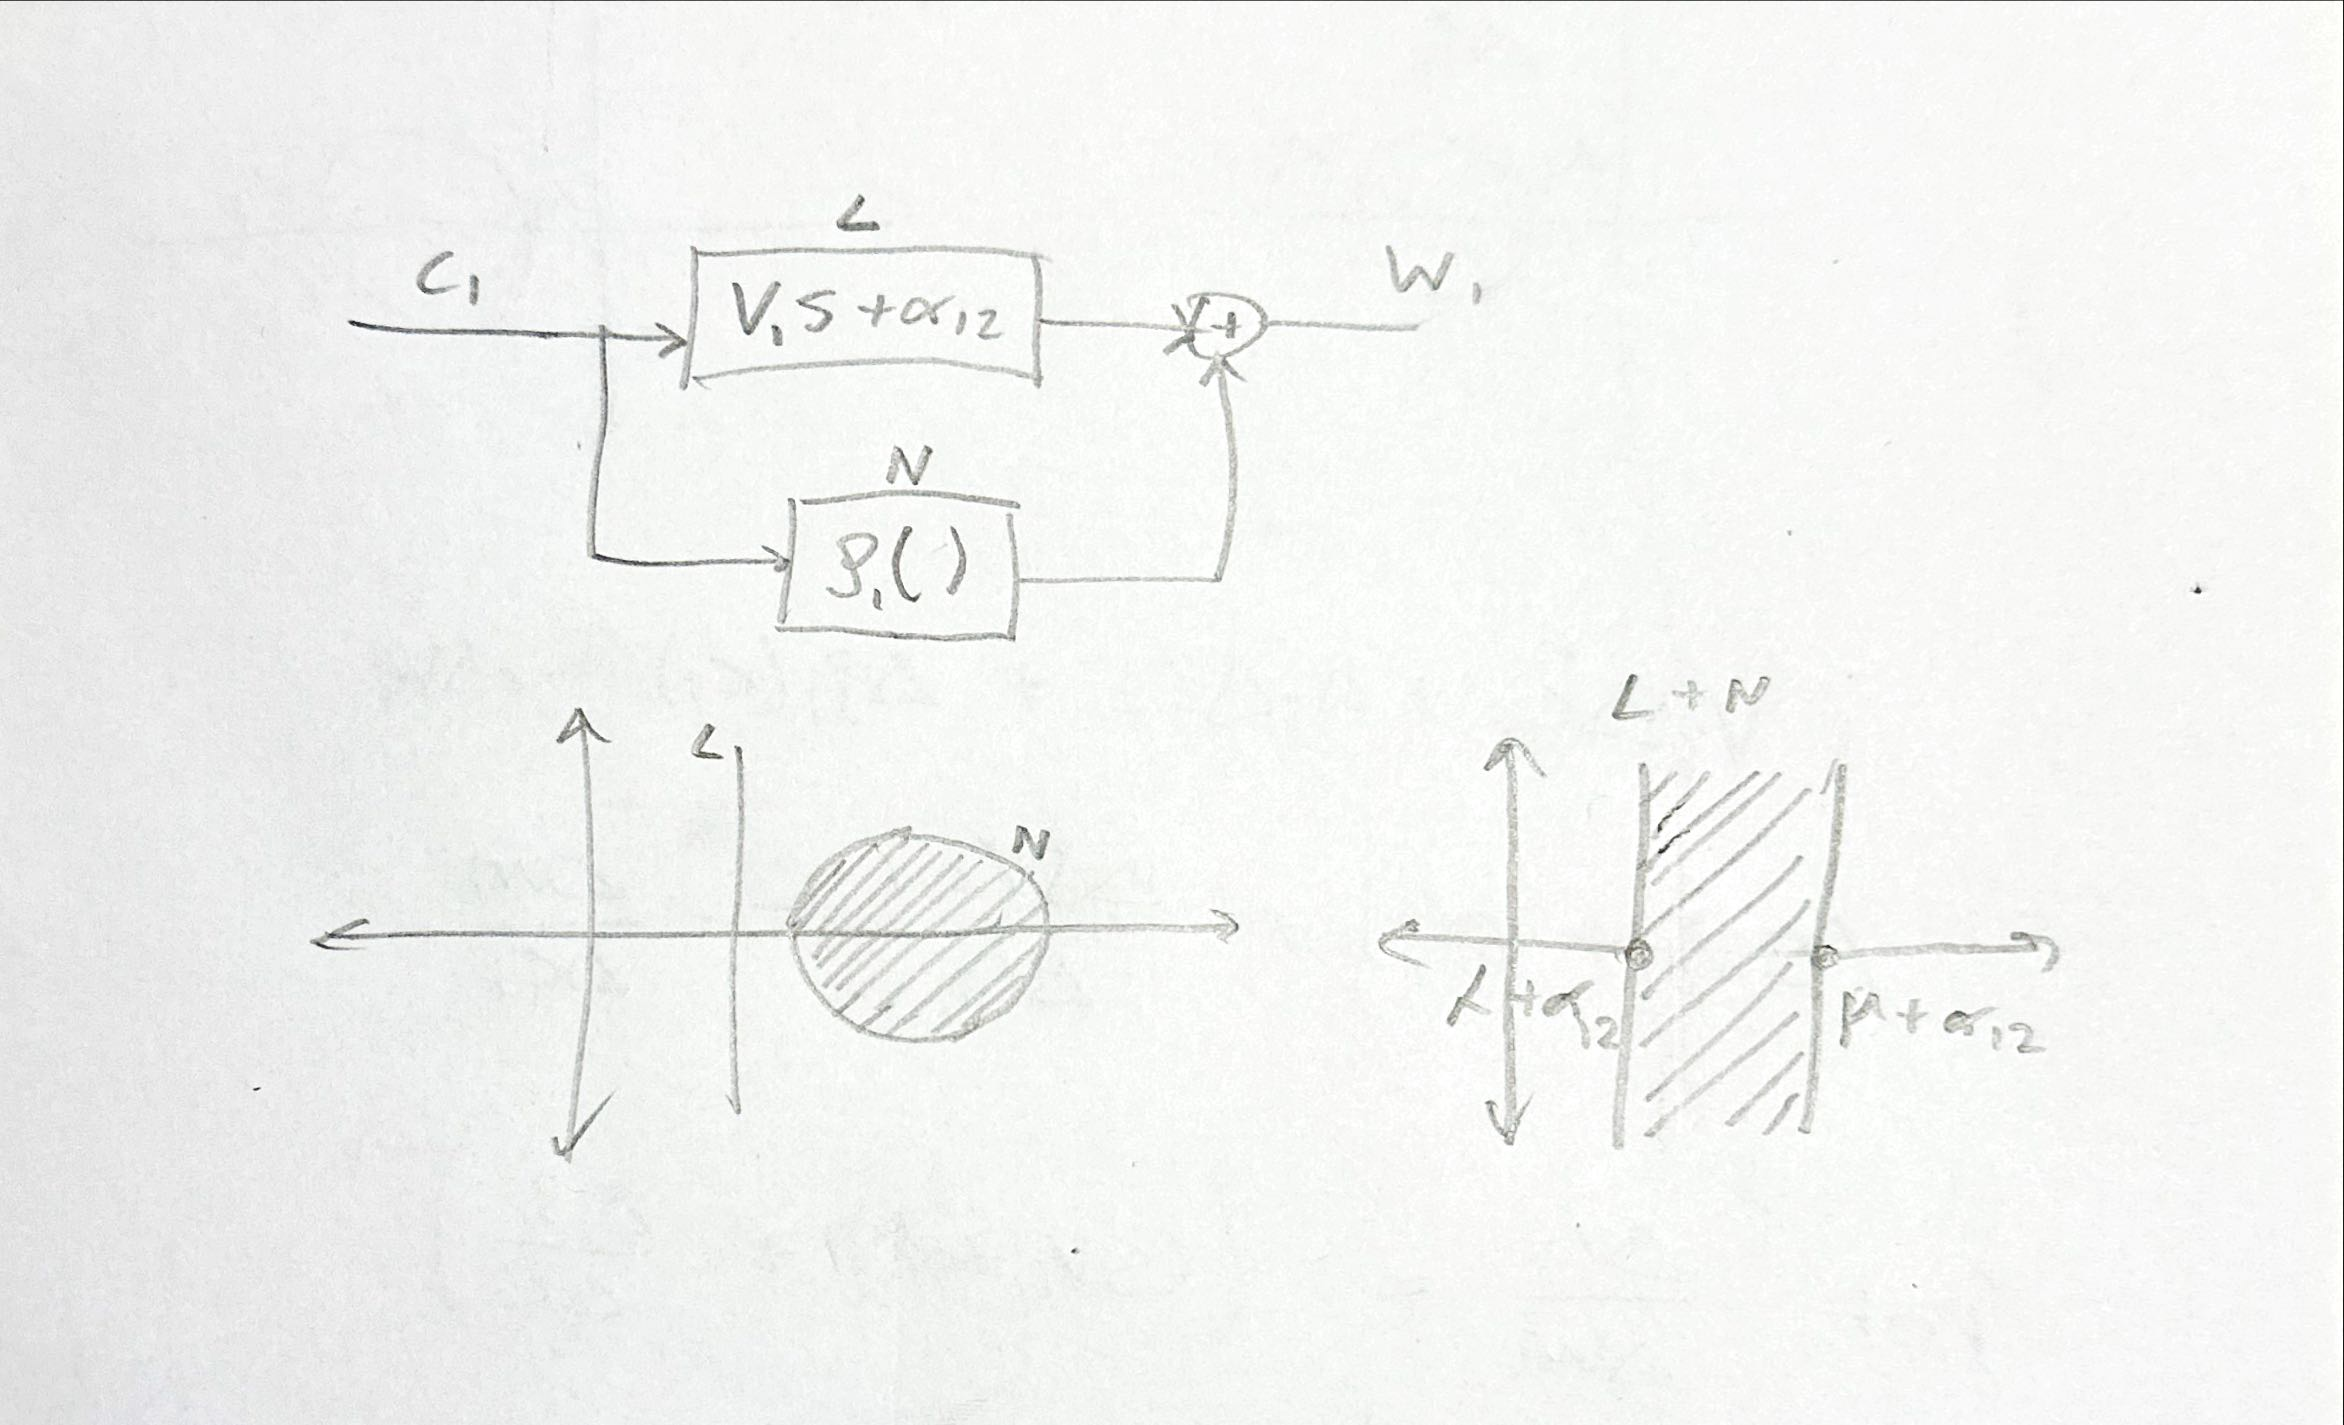
\includegraphics[width=0.4\textwidth]{figures/componentSRGs.jpg}
    \caption{Scaled Relative Graphs of sets L and N and their Minkowski sum}
\end{figure}
When inverted the resultant SRG is a larger circle between 0 and $1/(\lambda_1 + \alpha_{12})$ with a smaller circle removed from it between 0 and $1/(\mu_1 + \alpha_{12})$.
\begin{figure}[H]
    \centering
    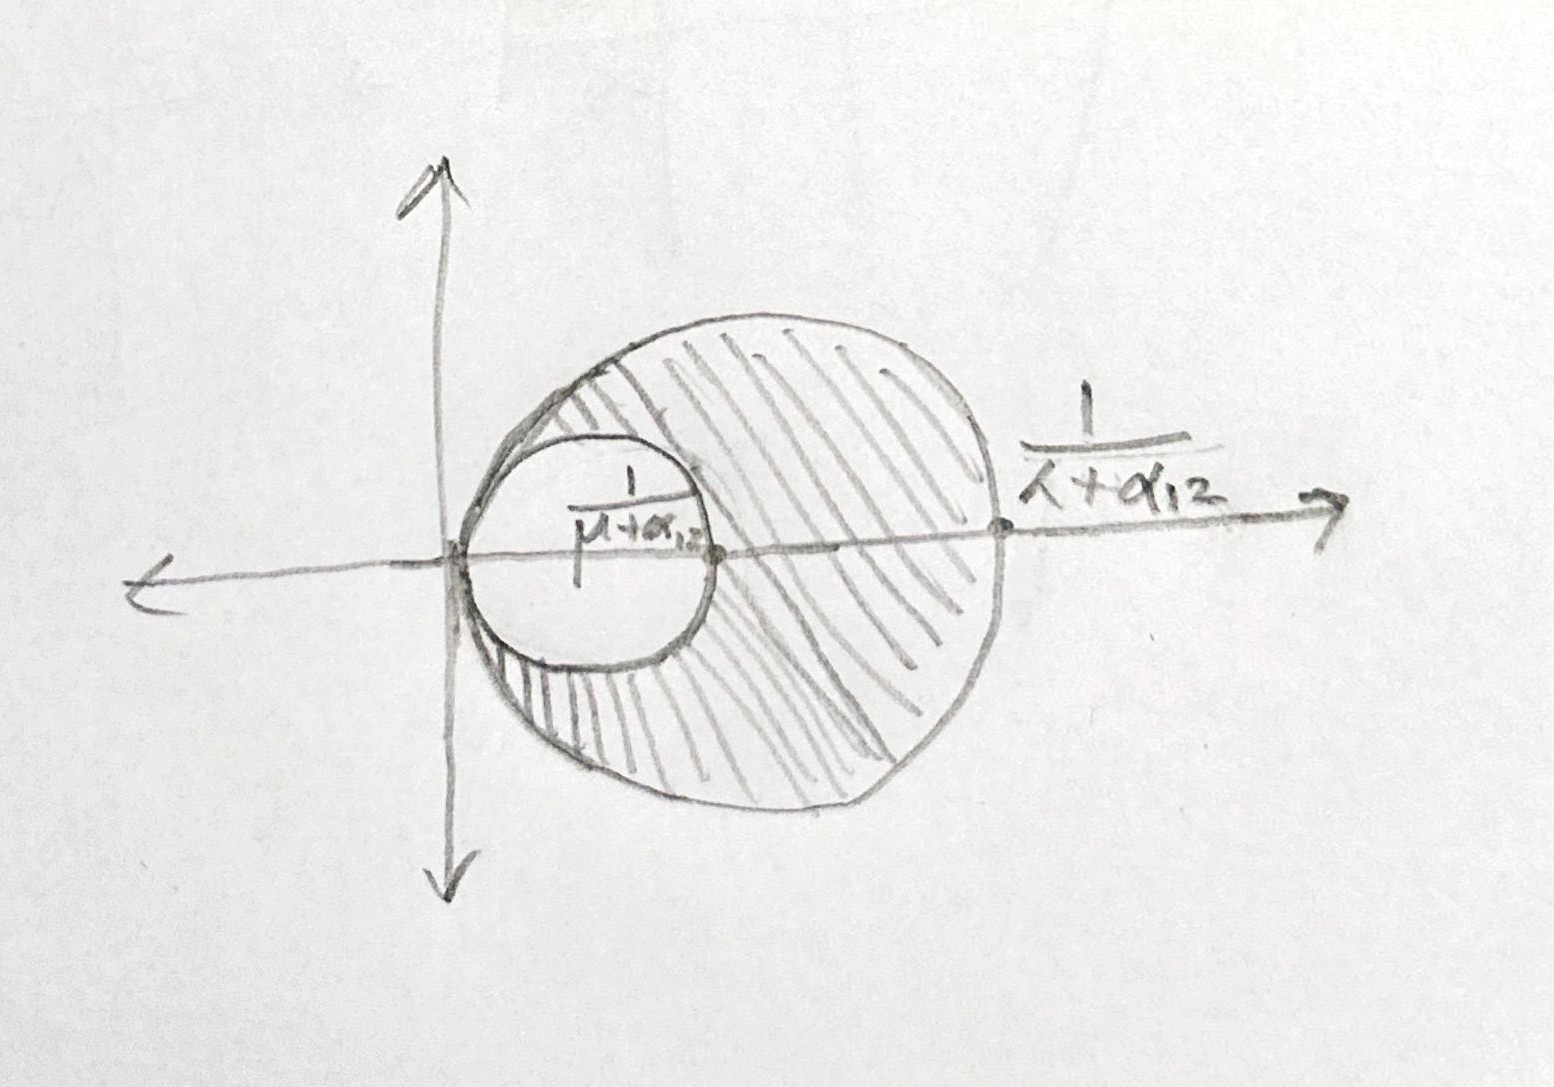
\includegraphics[width=0.4\textwidth]{figures/compartmentSRG.jpg}
    \caption{Scaled Relative Graph of component 1}
    \label{fig:compartment_srg}
\end{figure}

% Comment on the passivity and gain properties of this operator.
The SRG for one compartment, seen in figure \ref{fig:compartment_srg}, exists entirely in the right half plane and so is passive.
The gain properties inferred from passivity are that the gain is bounded which can also be seen from the SRG reaching a maximum of $1/(\lambda_1 + \alpha_{12})$ on the real axis.

\subsubsection{Positive feedback interconnection}

\begin{figure}[H]
    \centering
    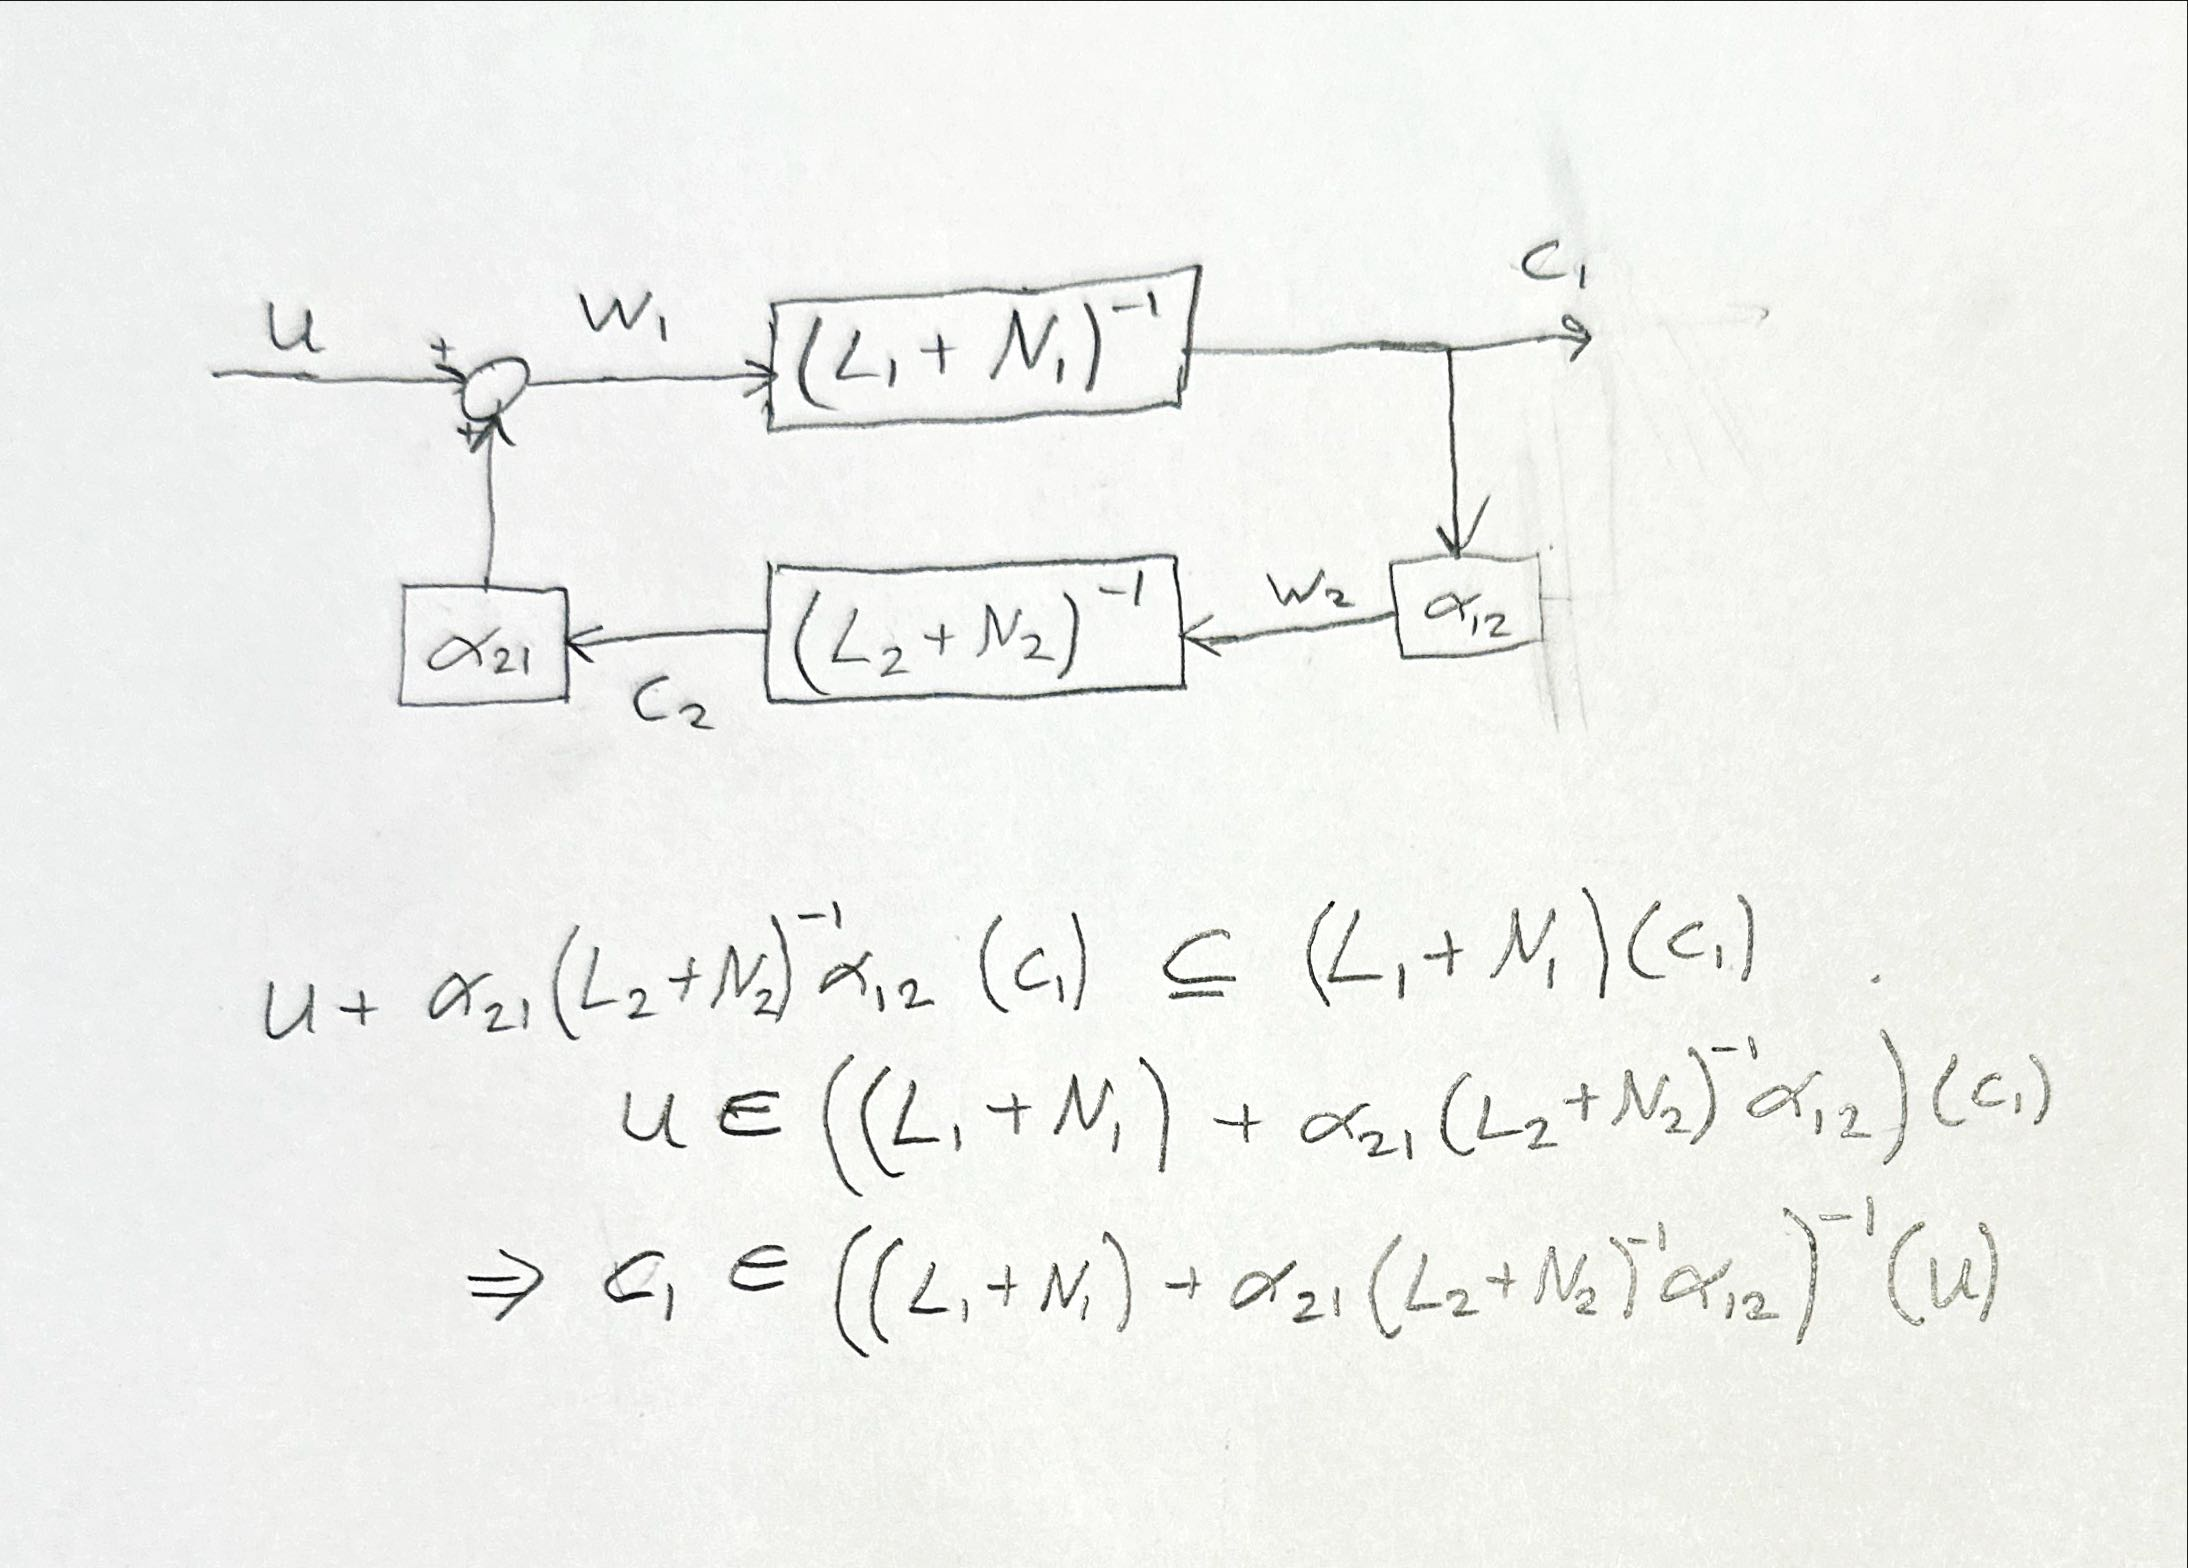
\includegraphics[width=0.4\textwidth]{figures/feedback_components.jpg}
    \caption{Derivation and diagram of the SRG }
\end{figure}

\begin{figure}[H]
    \centering
    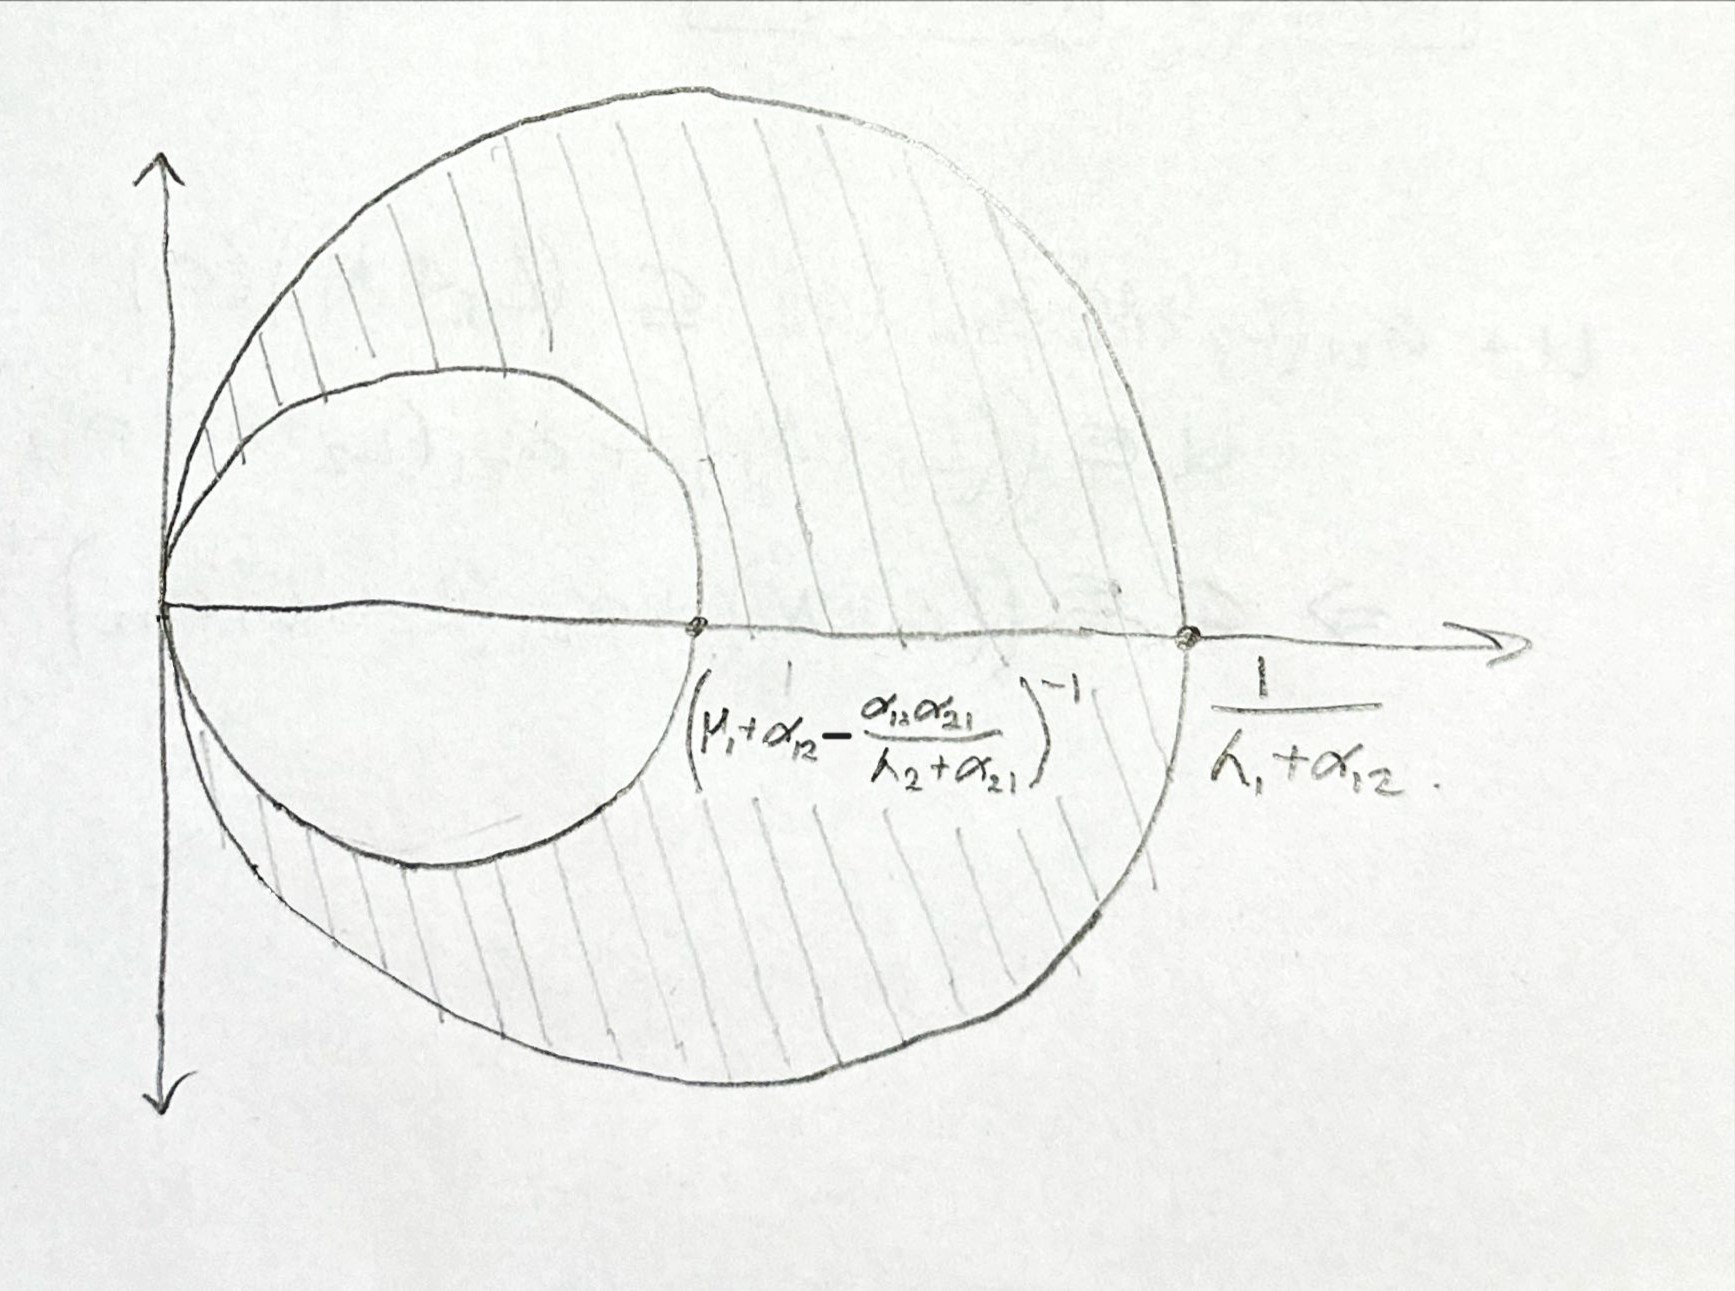
\includegraphics[width=0.4\textwidth]{figures/feedback_SRG.jpg}
    \caption{Scaled Relative Graph of positive feedback interconnection}
\end{figure}

\subsection{Automatic drug doses}

\subsubsection{Without sensor dynamics}

\begin{equation}
    u = k \text{ReLU}(r - y)
\end{equation}
\begin{equation}
    \text{ReLU}(x) = \begin{cases}
        x & \text{if } x > 0 \\
        0 & \text{otherwise}
    \end{cases}
\end{equation}
Which satisfies the incremental sector condition
\begin{equation}
    0 \leq k \frac{ReLU(x_1) - ReLU(x_2)}{x_1 - x_2} \leq k
\end{equation}

This means that the SRG of the controller can be represented by a disc between 0 and $k$.
The closed loop then consists of a cascade of the controller and plant.

\begin{figure}[H]
    \centering
    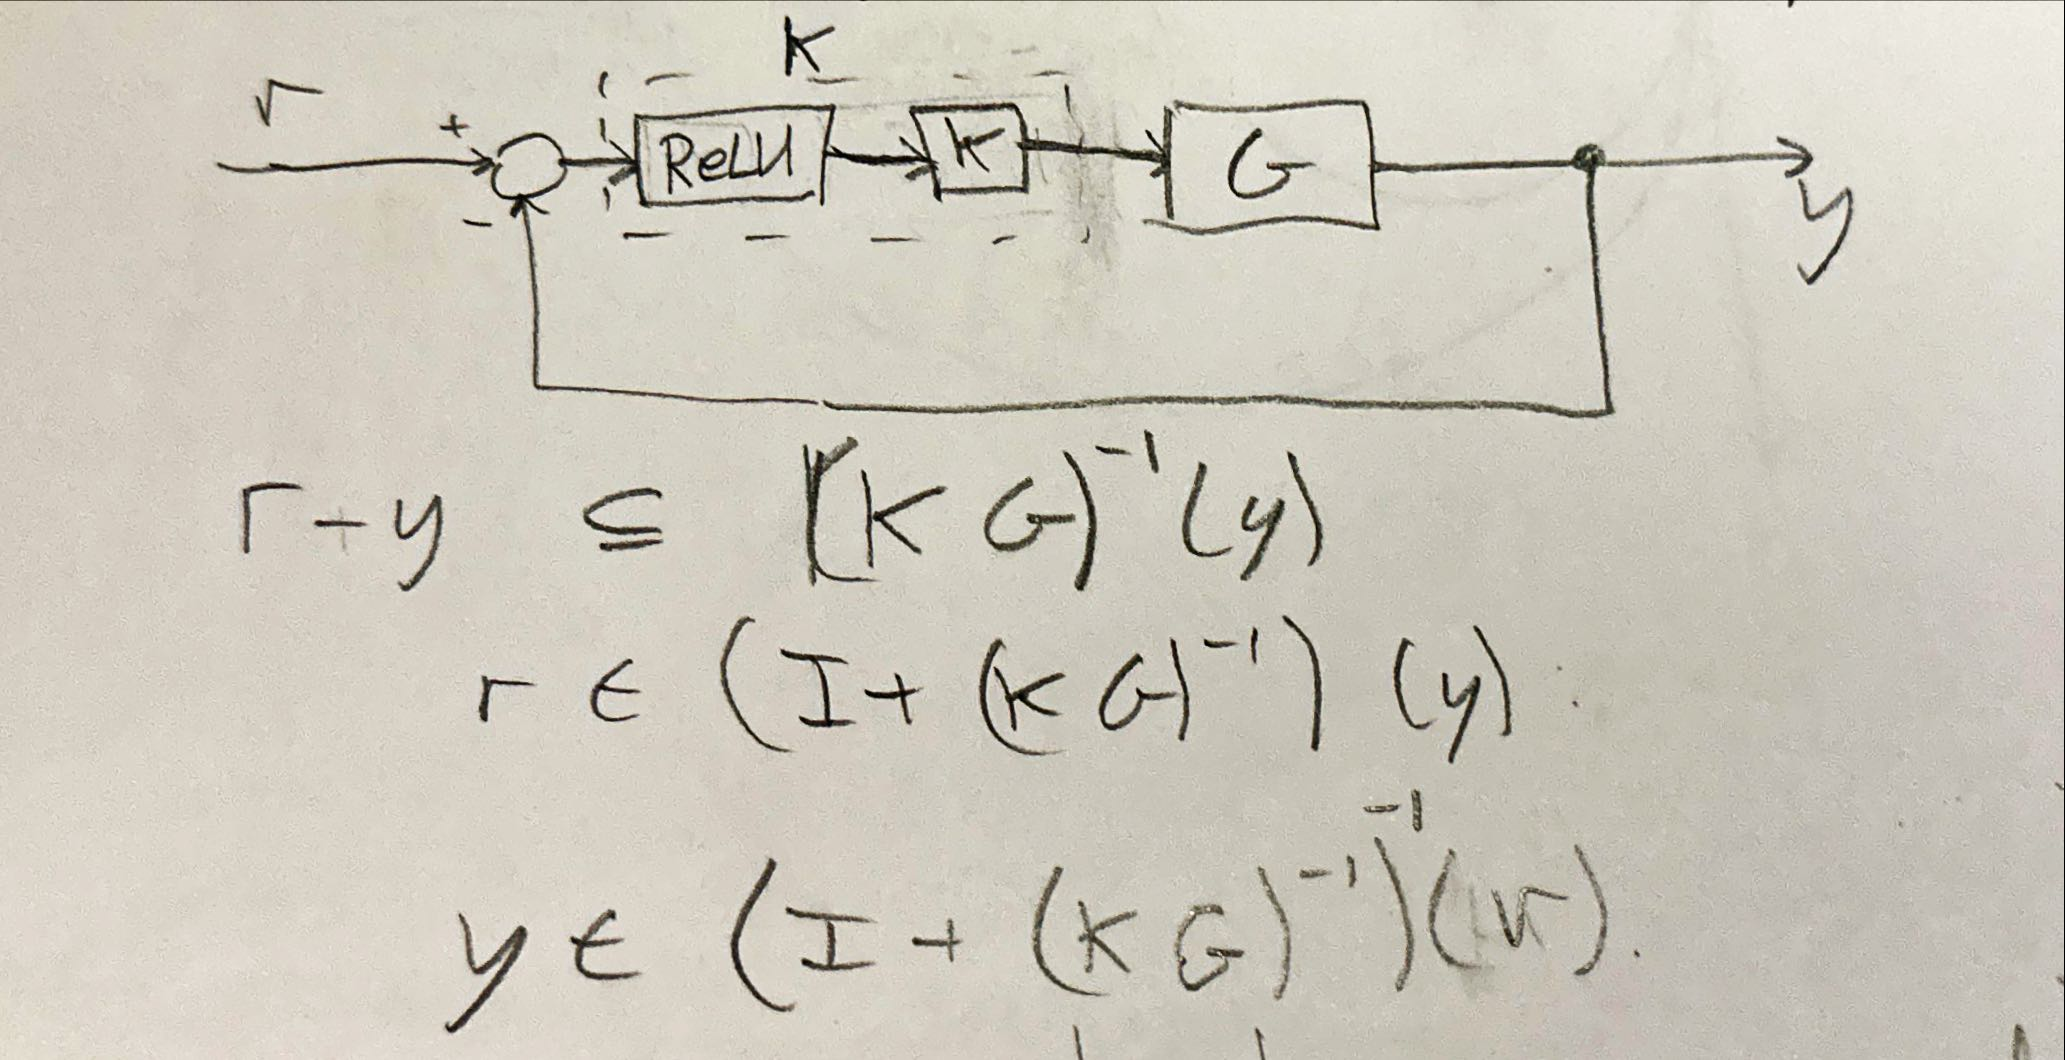
\includegraphics[width=0.6\textwidth]{figures/closed_loop.jpg}
    \caption{Closed loop block diagram}
\end{figure}
The SRG of the combined controller and plant forms a cardioid shape seen below.

\begin{figure}[H]
    \centering
    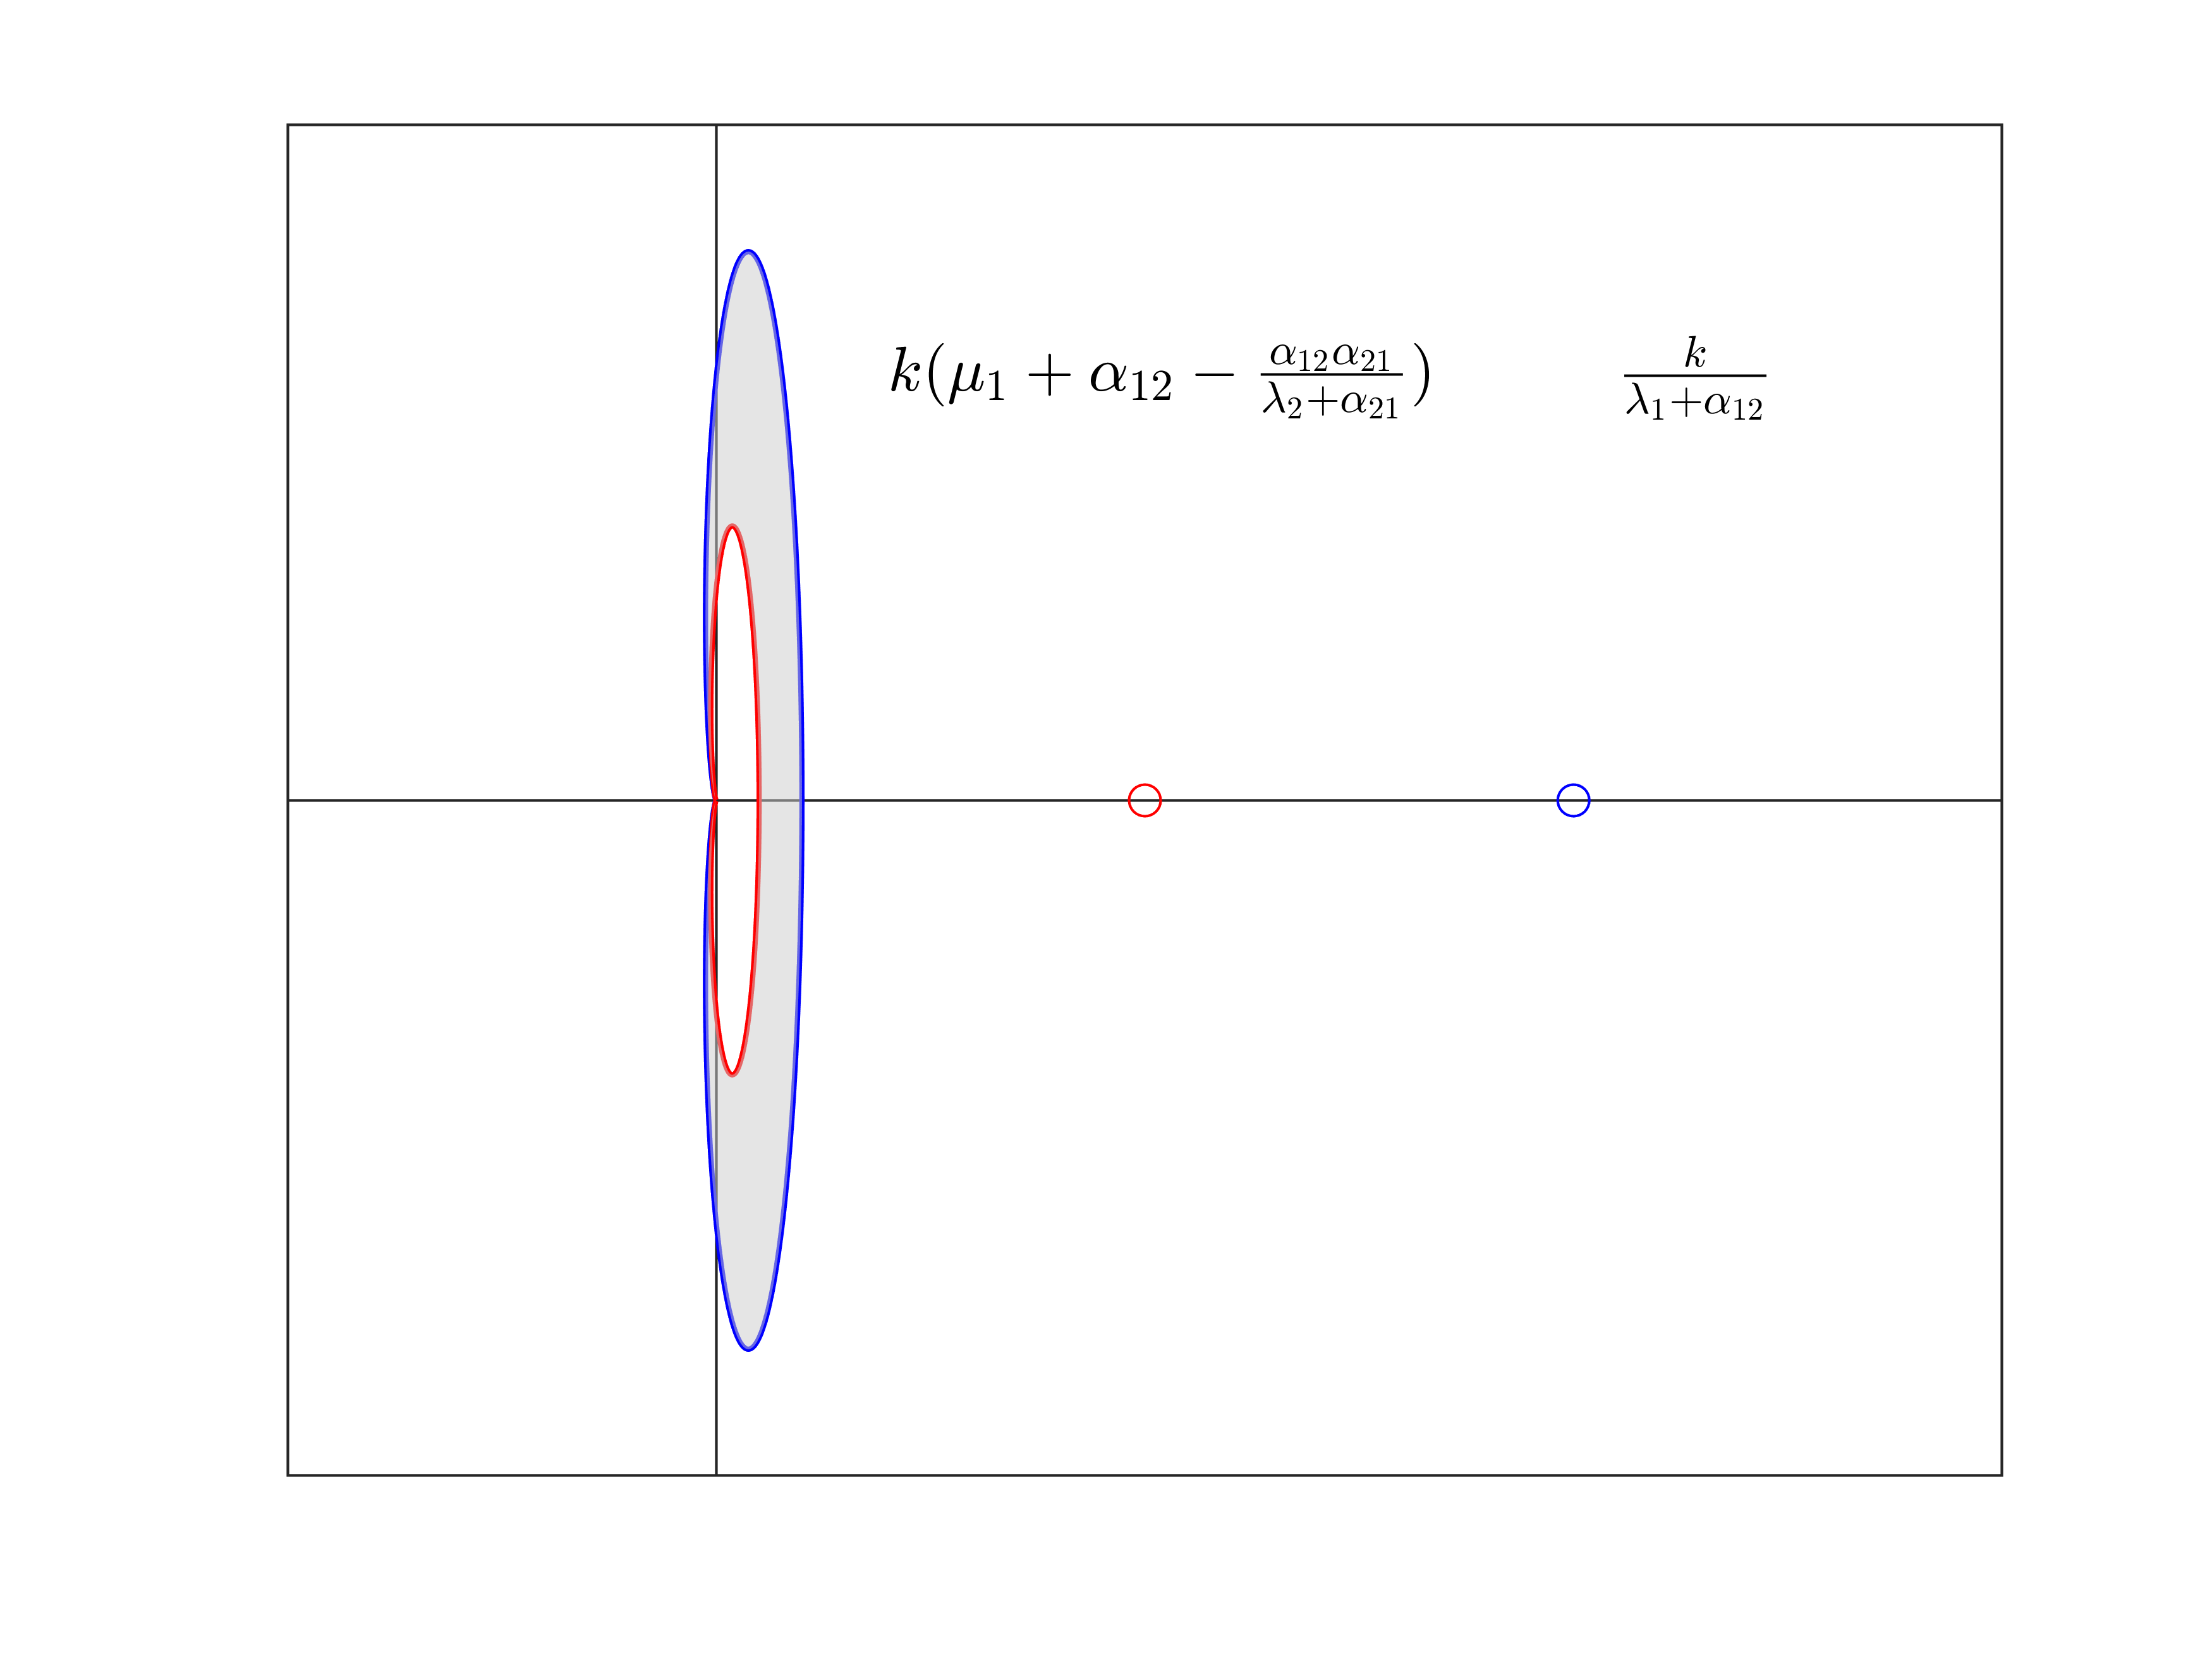
\includegraphics[width=0.6\textwidth]{figures/closed_loop_return_ratio.png}
    \caption{Scaled Relative Graph of closed loop return ratio}
    \label{fig:return_ratio_srg}
\end{figure}

For stability the Nonlinear Nyquist criterion is used.
%The closed loop system is stable if the number of encirclements of $-1$ by $kG(e^{j\theta})$ for $\theta \in [-\pi, \pi]$ equals the number of open loop unstable poles.
% should use the circle criterion.
%For determining the range of $k$ for stability, the Circle Criterion is used.
If $\text{SRG}(H_1^{-1})$ and -$\tau \text{SRG}(H_2)$ are separated by distance greater than $r_\text{min} > 0 \forall \tau \in [0,1]$.
Then the feedback interconnection of $H_1$ and $H_2$ has fading memory and incremental gain bound of $1/r_\text{min}$.
Considering $H_1$ as in figure \ref{fig:return_ratio_srg} and $H_2$ as 1 for $y=c_1$ means the distance from $H_1$ to the point $-\tau$.
This can be seen to satisfy the nonlinear Nyquist criterion for $k \geq 0$.

\subsubsection{With sensor dynamics}

The sensor has a time constant associated with it.

\begin{equation}
    \tau_s \dot{y} = -y + c_1
\end{equation}

This can be represented as an additional first order lag in the $H_2$ feedback interconnection.

\begin{figure}[H]
    \centering
    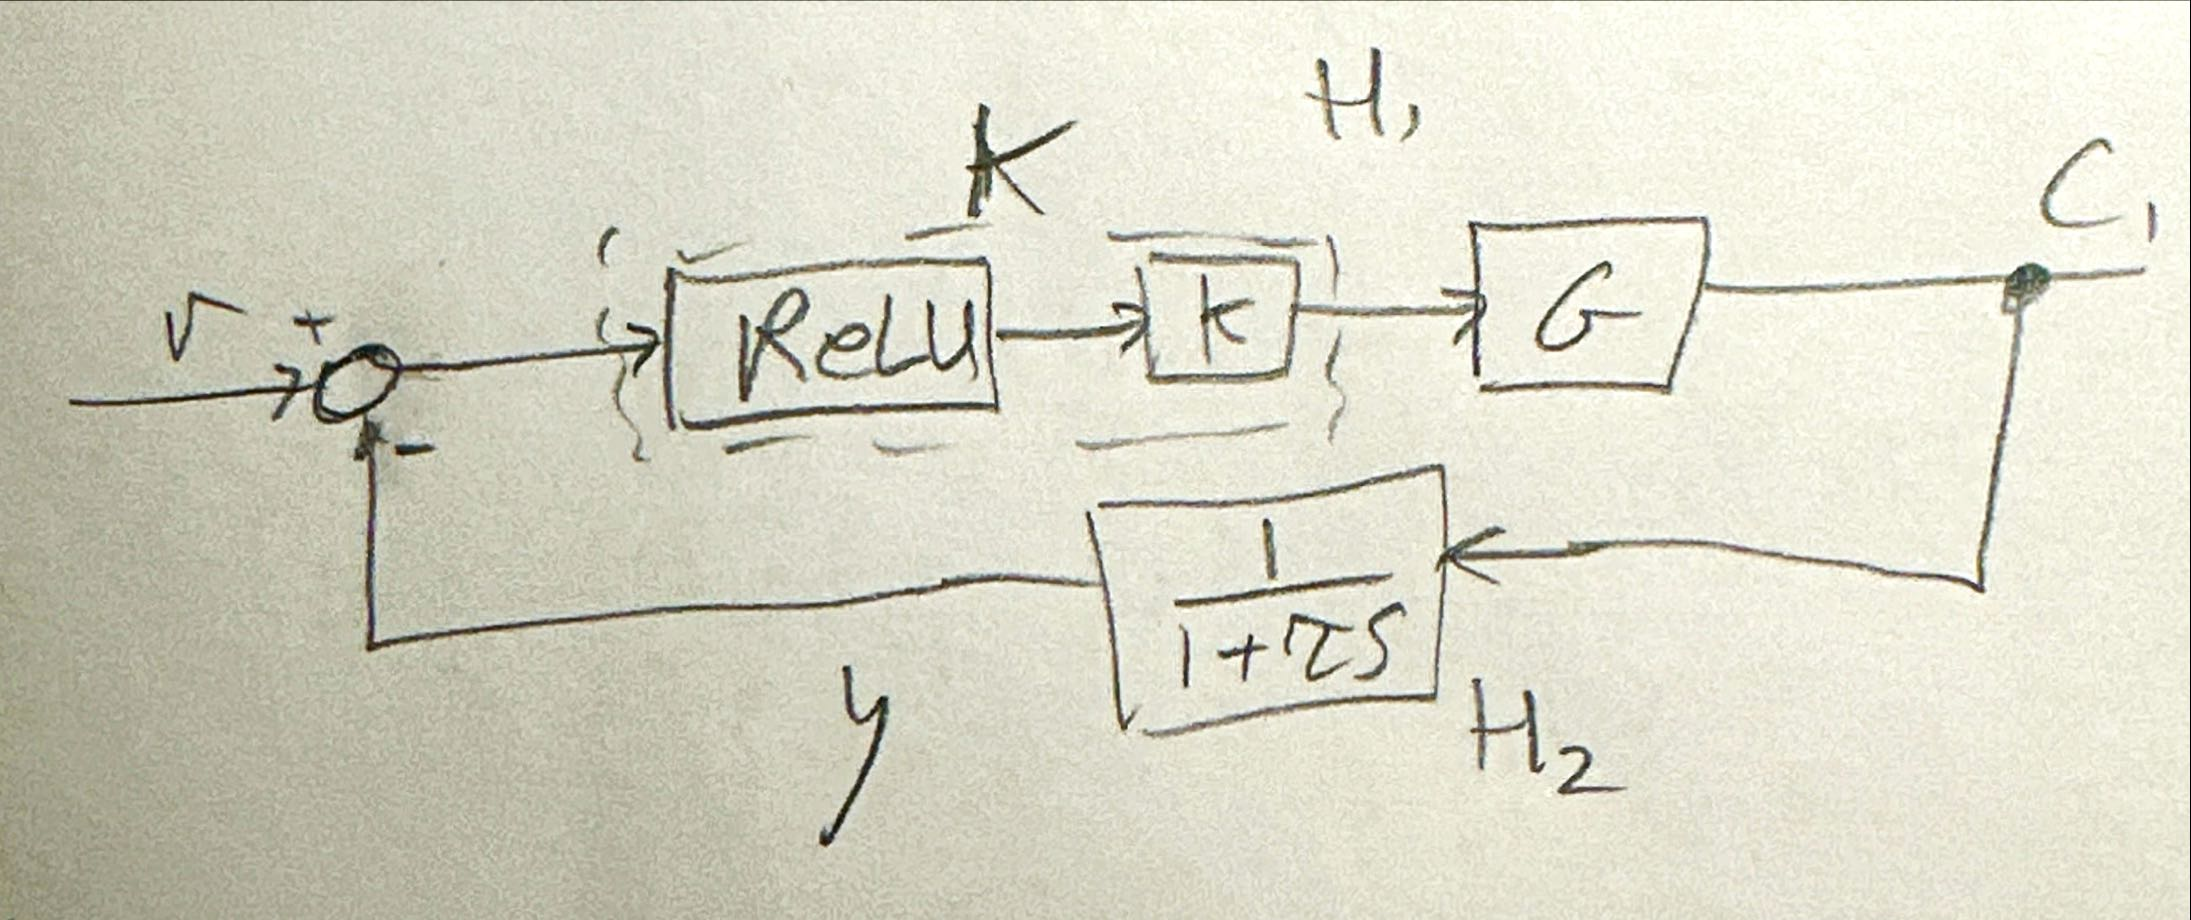
\includegraphics[width=0.6\textwidth]{figures/sensor_dynamics.jpg}
    \caption{Block diagram of system with sensor dynamics}
    \label{fig:sensor_dynamic_block}
\end{figure}

Both SRGs can be plotted and the minimum distance $r_\text{min}$ between $H_1$ and $-\tau H_2 $ for $\tau \in [0,1]$ can be calculated.
The point at which the SRGs intersect is the point at which the system becomes unstable and the maximum bound on $k$ can be found.

% TODO: find the right answer for this
% somethings gone wrong earlier because for all tau>0 the SRGs overlap

\subsection{Advanced sensor delay and describing function method}

A more accurate model of the sensor dynamics is given by the following differential equation:
\begin{align}
    10\dot{x} &= -x + c_1 \\
    y(t) &= x(t-0.1)
\end{align}

A pure time delay can still be represented as a linear system which can be seen in the laplace domain below:
\begin{align}
    (10s + 1)x &= c_1 \\
    y(t) &= x \cdot e^{-0.1s}
\end{align}

The ReLU function for an injected sinusoidal input $E\sin(\omega t)$ 
\begin{equation}
    u(t) = k \text{ReLU}(E\sin(\omega t)) = k \cdot \begin{cases}
        E\sin(\omega t) & \text{if } E\sin(\omega t) > 0 \\
        0 & \text{otherwise}
        \end{cases}
\end{equation}
Which takes the form of a half-wave rectified sine wave.

\begin{equation}
    N(E) = \frac{1}{\pi E} \int_0^\pi E \sin^2(\theta) d\theta = \frac{1}{2}
\end{equation}
This means that the describing function of ReLU simply attenuates the input by a factor of 1/2.

The time delayed system was simulated in Matlab using the delayed differential equation solver \texttt{dde23}.
Due to time constraints the describing function limit cycle was not simulated.

\begin{figure}[H]
    \centering
    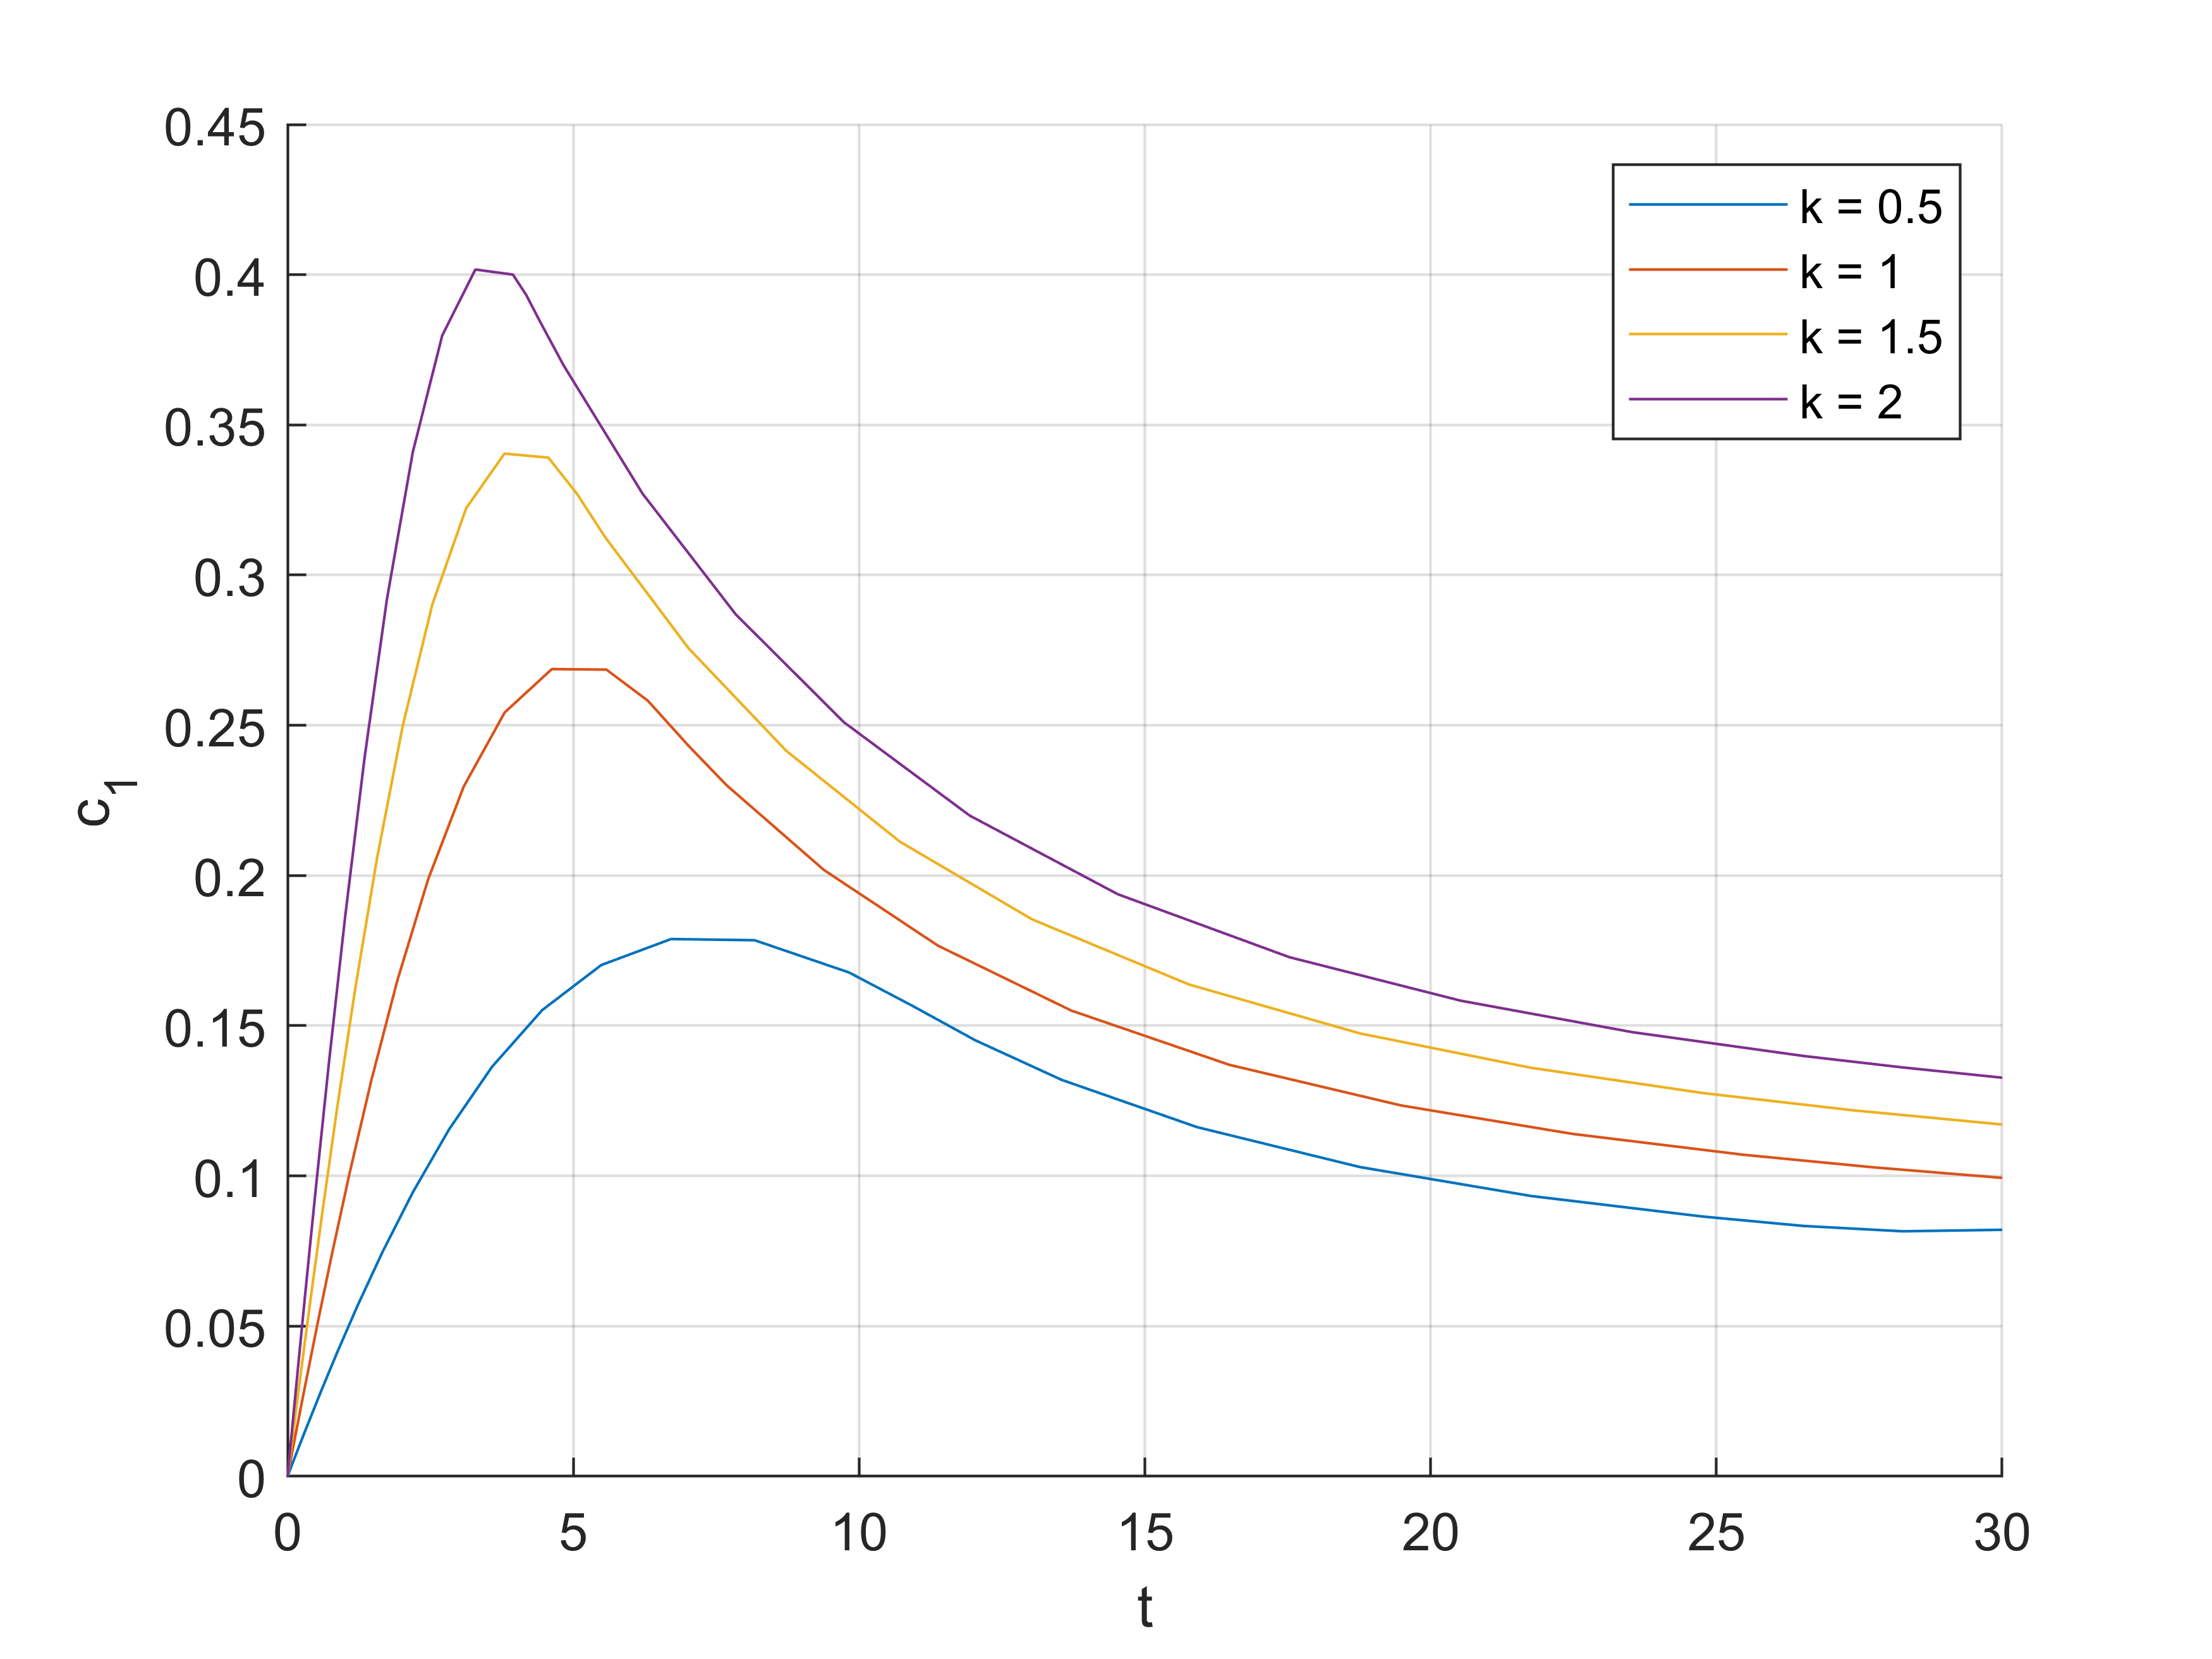
\includegraphics[width=0.6\textwidth]{figures/23_pharmacokinetic_sim.png}
    \caption{Simulation of the pharmacokinetic system with delayed sensor dynamics}
    \label{fig:pharmacokinetic_sim}
\end{figure}

\section{Appendix}

\begin{figure}[H]
    \centering
    \begin{lstlisting}
        cvx_begin sdp
            variable Y(3,3) symmetric
            variable Z(1,3)
            variable epsl
            
            minimise(epsl)

            LMI1 = Y >= 0;
            LMI2 = epsl >= 0;
            
            LMI3 = [ Y*df'+df*Y + 2*lamda*Y + epsl*eye(3), Bw, Y*C';
                    Bw', -gama*eye(1), Dw';
                    C*Y, Dw, -gama*eye(1) ] <= 0;
            
            LMI4 = [ Y*df'+df*Y + 2*lamda*Y + epsl*eye(3) + Z'*Bu' + Bu*Z, Bw, Y*C';
                    Bw', -gama*eye(1), Dw';
                    C*Y, Dw, -gama*eye(1) ] <= 0;
                
        cvx_end
    \end{lstlisting}
    \caption{CVX code for bounded differential gain in i)}
    \label{fig:bounded_differential_gain_lmi}
\end{figure}

\begin{figure}[H]
    \centering
    \begin{lstlisting}
        cvx_begin sdp
                variable Y(n,n) symmetric
                variable Z(1,n)
                variable epsilon
                
                minimize( eps )
                
                LMI1 = epsilon >= 0;
                
                LMI2 = df*Y + Y*df' + 2*lamda*Y + Z'*Bu' + Bu*Z + eps*eye(n) <= 0;
                LMI3 = df*Y + Y*df' + 2*lamda*Y + eps*eye(n) <= 0;
                
                LMI4 = Y*df' + df*Y + Z'*Bu'+Bu*Z+eps*eye(3) <= 0;
                
        cvx_end
    \end{lstlisting}
    \caption{CVX code for enforced 2-dominance and instability of 0 equilibrium in iii)}
    \label{fig:enforced_2_dominance_lmi}
\end{figure}

\begin{figure}[H]
    \centering
    \begin{lstlisting}
        cvx_begin sdp
            variable P(2,2) symmetric
            variable alph
            variable epsilon

            minimize(epsilon)

            LMI1 = alph >= 0;

            LMI2 = epsilon >= 0;
                    
            LMI3 = [A1'*P + P*A1 + 2*lamda*P - alph*(C')*C + epsilon*eye(2), P*B-C';
                    B'*P-C, -betaa*eye(1)] <= 0;

            LMI4 = [A2'*P + P*A2 + 2*lamda*P - alph*(C')*C + epsilon*eye(2), P*B-C';
                    B'*P-C, -betaa*eye(1)] <= 0;
        
        cvx_end
    \end{lstlisting}
    \caption{CVX code for determining excess output passivity of insect wing model in iv)}
    \label{fig:determining_excess_output_passivity_lmi}
\end{figure}

\begin{figure}[H]
    \centering
    \begin{lstlisting}
        
        cvx_begin sdp
            variable Y(n,n) symmetric
            variable Z(1,n)
            variable epsilon

            minimize(epsilon)

            LMI1 = epsilon >= 0;
            
            LMI2 = [ (Y*df' + df*Y + 2*lamda*Y + Z'*Bu' + Bu*Z + epsilon*eye(n)),   (Bw - Y*C');
                    (Bw' - C*Y),                                (-(Dw + Dw') - betaa2*eye(1))] <= 0;
                
            LMI3 = [ (Y*df' + df*Y + 2*lamda*Y + epsilon*eye(n)),   (Bw - Y*C');
                    (Bw' - C*Y),                                (-(Dw + Dw') - betaa2*eye(1))] <= 0;
            
            LMI4 = Y*df' + df*Y + Z'*Bu'+Bu*Z + epsilon*eye(3) <= 0;

        cvx_end
    \end{lstlisting}
    \caption{CVX code for designing weights with equivalent shortage input passivity in iv)}
    \label{fig:equivalent_shortage_input_passivity_lmi}
\end{figure}


\begin{thebibliography}{9}

    %Endres, SC, Sandrock, C, Focke, WW (2018) “A simplicial homology algorithm for lipschitz optimisation”, Journal of Global Optimization.
    
      \bibitem{handout}
      F. Forni, R, Sepulchre
      \emph{4F2, Robust and Nonlinear Control: Coursework 1}
      University of Cambridge,
      2025.

      \bibitem{lecture}
      F. Forni
      \emph{4F2, Robust and Nonlinear Control: Handout 6}
      University of Cambridge,
      2025.
    
      \bibitem{matlab_robustmu}
      MATLAB
      \emph{Robust Performance Measure for Mu Synthesis}
      \texttt{https://uk.mathworks.com/help/robust/ug/measures-of-robust-performance.html}

    
\end{thebibliography}

\end{document}